\documentclass[a4paper,10pt]{scrartcl}
\usepackage[utf8x]{inputenc}
\usepackage{amsthm,amssymb,amsmath}
\usepackage{ulem}
\usepackage{graphicx}
\usepackage{pdfpages}
\usepackage[german]{babel}
\usepackage{color}
\usepackage{subfigure}
\usepackage{wasysym}
\usepackage{ulsy}

%definition of new enviroments
\newtheorem*{bemerkung*}{Bemerkung}
\newtheorem*{definition}{Definition}
\newtheorem*{definition*}{Definition}
\newtheorem*{bezeichnungen}{Bezeichnungen}
\newtheorem*{fakt}{Fakt}
\newtheorem*{beispiel}{Beispiel}
\newtheorem*{beispiel*}{Beispiel}
\newtheorem*{satz}{Satz}
\newtheorem*{satz*}{Satz}
\newtheorem*{lemma}{Lemma}
\newtheorem*{protokoll*}{Protokoll}
\newtheorem*{idee}{Idee}

%definition of new commands
\newcommand{\DGEF}{\text{\textbf{DGEF}}}

%opening
\title{Cake-Cutting-Algorithms\\or\\What you can learn from an Ass}
\author{Prof. J. Rothe}

\begin{document}

\maketitle

 \begin{abstract}
% %  \begin{arrows_theorem}
% %   There is no nondictactorial social welfare function satisfying Pareto-optimality and independece of irrelevant alternatives.
% %  \end{arrows_theorem}

 \begin{center}
  \begin{figure}
  \subfigure{\includegraphics[height=0.29\textheight]{fig/rothe_scotch.png}}\hfill
  \subfigure{\includegraphics[height=0.28\textheight]{fig/frog.png}}
  \end{figure}
 \end{center}
 \end{abstract}

\newpage
\section*{}
 \begin{itemize}
  \item[ \underline{Der Kuchen:}] \includegraphics[height=0.05\textheight]{01Kuchen}
  \item[ \underline{Die Spieler:}] \xout{Alice}, \xout{Bob}, C$_{laudia}$, D$_{oro}$, E$_{dith}$, F$_{elix}$, G$_{abor}$ oder 
       $p_1,p_2,\ldots,p_n$
  \item[ \underline{Das Ziel:}] Gerechte Aufteilung 
 \end{itemize}

\section{Einführung in gerechte Kuchenaufteilung}
 \begin{itemize}
  \item[Fairness:] ``persönlich'', ``gefühlt'' $\rightarrow$ nötig: (formale) Axiomatisierung
  \item[Kuchen:] inhomogene Ressource
  \item[Spieler:] Jeder hat individuelle Bewertung der einzelnen Stücke, die privat ist
 \end{itemize}                                                                          
 \includepdf[pages=3-6,nup=2x2]{folien.pdf}
\subsection{Methoden für zwei Spieler}
 \begin{itemize}
  \item[\underline{Methode 1:}] \begin{tabular}{cc}
                                 $v_M(1)=50\%$ & $v_M(2)=50\%$\\
                                 $v_C(1)=80\%$ & $v_C(2)=20\%$\\
                                 $v_F(1)=40\%$ & $v_F(2)=60\%$
                                \end{tabular}
  \item[\underline{Methode 2:}] \underline{garantiert}(in jeder Bewertung der Spieler) keinem Spieler $\geq50\%$, $\geq10\%$
  \item[\underline{Methode 3:}] unfair, da C das Stück von F bestimmen kann
  \item[\underline{Methode 4:}] Cut \& Choose: \begin{itemize}
                                               \item[]Cutter: genau 50\%
                                               \item[]Chooser: $\geq50\%$ ($>50\%$ bei verschiedenen Bewertungen) 
                                              \end{itemize}
 \end{itemize}
\includepdf[pages=7-8,nup=2x1]{folien.pdf}
\subsection{Drei Spieler: Ein falscher Start}
 \underline{Ziel:} Jeder Spieler soll einen proportionalen Anteil (hier: $\frac{1}{2}$) bekommen\\
 Wer ist zufrieden?
 \begin{itemize}
  \item Edith bestimmt, da sie zuerst wählt und eines von $X_1$, $X_{2,1}$, $X_{2,2}$ hat den Wert $v_E(\cdot)\geq\frac{1}{3}$
  \item Claudia ist auch zufrieden, denn ihr Schnitt ist so, dass $v_C(X_1)=\frac{1}{3}\Rightarrow$ egal wie Doro schneidet, 
        gilt für mindestens eins von $X_{2,1}$ und $X_{2,2}: v_C(\cdot)\geq\frac{1}{2}\cdot v_C(X_2)=\frac{1}{2}\cdot\frac{2}{3}=
        \frac{1}{3}$ und sie wählt als Zweite 
        \begin{bemerkung*} 
         $v_C(X_1)<\frac{1}{3}\Rightarrow X_1$ nicht akzeptabel und wenn eines von $X_{2,1}$ und $X_{2,2}$ nicht erfüllt:
         $v_C(\cdot)\geq\frac{1}{3}$ dann ist nur ein Stück akzeptabel für C. Da sie als Zweite wählt, ist ihr dieses Stück nicht sicher.
         $v_C(X_1)>\frac{1}{3}\Rightarrow v_C(X_2)<\frac{2}{3}$ und wenn D so schneidet, dass $v_C(X_{2,1})=v_C(X_{2,2})<\frac{1}{3}$
         Wieder ist nur ein Stück für C akzeptabel, aber nicht sicher
        \end{bemerkung*}
  \item Doro ist nicht garantiert zufrieden, sondern nur, wenn sie mit C's Schnitt über\-einstimmt: $v_C(X_1)=v_D(X_1)=\frac{1}{3}$\\
        Weil D $X_2$ selbst schneidet wären für sie drei Stücke akzeptabel. Aber wenn $v_D(X_1)\neq\frac{1}{3}$, sind nur zwei Stücke
        für sie ok. \\
        $v_D(X_1)<\frac{1}{3}: X_{2,1},X_{2,2}$ ok, $X_1$ nicht\\
        $v_D(X_1)>\frac{1}{3}: X_1$ ok, aber höchstens eins von $X_{2,1},X_{2,2}$\\
        (Bsp.: $v_D(X_1)=70\%\Rightarrow v_D(X_2)=30\%$, so ist weder $X_{2,1}$ noch $X_{2,2}$ ok)
 \end{itemize}

\subsection{proportionale Aufteilung für n Spieler}
 \begin{itemize}
  \item[Kuchen:] $X=[0,1]$ reelles Einheitsintervall
  \item[Stück:] $[x,y]\subseteq[0,1]$
  \item[Spieler:] $p_1,p_2,\ldots,p_n$ bewerten alle Stücke, wobei i.A. ``Wert''$\neq$``Größe'' (Kuchen inhomogen)
 \end{itemize}
 Jeder Spieler $p_i$ hat ein Maß (Bewertungsfunktion)
 \begin{displaymath}
  v_i:{X'|X'\subseteq X}\rightarrow[0,1]\subset\mathbb{R}
 \end{displaymath}
 das $v_i(\emptyset)=0$ und $v_i(X)=1$ und einige weitere Axiome (kommen später) erfüllt.
 \begin{definition}
  Eine Aufteilung des Kuchens $X=\bigcup\limits_{i=1}^{n}X_i$, wobei $X_i$ die Portion von Spieler $p_i$ ist, heißt
  \underline{proportional}, falls für alle $i$, $1\leq i\leq n$,
  \begin{displaymath}
   v_i(X_i)\geq\frac{1}{n}
  \end{displaymath}
  gilt und heißt \underline{überproportional}, falls für alle $i$, $1\leq i\leq n$
  \begin{displaymath}
   v_i(X_i)>\frac{1}{n}
  \end{displaymath}
  gilt.\\
  Ein Cake-Cutting-Protokoll(CCP) heißt \underline{proportional} (bzw. \underline{überproportional}), falls es unabhängig
  von den Maßen der Spieler eine proportionale (bzw. überproportionale) Aufteilung garantiert, sofern sich alle Spieler an die
  Regeln und die Strategien des Protokolls halten.
 \end{definition}
 \begin{bezeichnungen}
  \begin{tabular}{rcl}
   proportional &$\hat{=}$& ``simple fair'' (simpel fair)\\
   überproportional &$\hat{=}$& ``strongly fair''
  \end{tabular}
 \end{bezeichnungen}
 \begin{fakt}
  Das Cut \& Choose Protokoll ist proportional
 \end{fakt}
\includepdf[pages={10,9},nup=2x1]{folien.pdf}
 \begin{beispiel}Moving-Knife-Protokoll für C,D,E
  \begin{itemize}
   \item[] Angenommen D schreit zuerst ``Halt!'' und erhält $X_1$\\
           $\Rightarrow v_D(X_1)=\frac{1}{3}$, also ist für $X_2=X-X_1$\\
           $v_C(X_2)\geq\frac{2}{3}$ und $v_E(X_2)\geq\frac{2}{3}$, weil sie noch nicht gerufen haben
   \item[] Jetzt schreit E ``Halt!'' $\Rightarrow$ E erhält $X_{2,1}$ mit
           \begin{align*}
            v_E(X_{2,1})=\frac{1}{2}v_E(X_1)\geq\frac{1}{2}\cdot\frac{2}{3}=\frac{1}{3}
           \end{align*}
   \item[] Da C noch nicht gerufen hat, ist für $X_{2,2}=X-(X_1\bigcup\limits X_{2,1})$
           \begin{align*}
            v_C(X_{2,2})\geq\frac{1}{3}
           \end{align*}
  \end{itemize}
  \begin{fakt}
   Das Moving-Knife-Protokoll ist proportional
  \end{fakt}
  \begin{bemerkung*}
   \begin{itemize}
    \item Tie-Breaking-Rule: Rufen mehrere Spieler gleichzeitig ``Halt!'', so kann das Stück beliebig zugewiesen werden
    \item Wenn ein Spieler ``strategisch'' spielt, also nicht bei $\frac{1}{n}$, sondern erst bei $\frac{1}{n-\varepsilon}$,
          $0<\varepsilon\leq n-1$, ruft (z.B. nicht bei $\frac{1}{3}$, sondern bei $\frac{1}{2}$) dann riskiert er seinen
          proportionalen Anteil (z.B. wenn jemand anders bei 0,4 ruft)
    \item Die letzten beiden Spieler könnten gefahrlos nach $\frac{1}{2}$ des Restkuchens abwarten, bis beide Reststücke gleichwertig sind
   \end{itemize}
  \end{bemerkung*}
  Wesentlicher Nachteil des Moving-Knife-Protokolls:\\
  Es müssen von jedem Spieler überabzählbar viele Entscheidungen getroffen werden: jede für eine Messerposition, in einem Kontinuum von 
  Positionen
 \end{beispiel}
\includepdf[pages=11,scale=0.8]{folien.pdf}
\begin{fakt}
 Das Last-Diminisher-Protokoll ist proportional
\end{fakt}
\begin{proof}
 In jeder Runde erhält ein Spieler seine Portion (in der letzten Runde: 2) und scheidet aus.\\
 Sei $\bar {p}_1,\bar{p}_2,\ldots,\bar p_n$ die Reihenfolge in der die Spieler ausscheiden. In Runde $i\leq n-1$ sind noch $\bar p_i,
 \bar p_{i+1},\ldots,\bar p_n $ und der Rest $R_i=X-\bigcup\limits_{j<i}X_i$ im Spiel, wobei $X_i$ die Portion von $\bar p_i$ und 
 $\bar v_i$ das Maß von $\bar p_i$ ist.
 \begin{description}
  \item[Runde 1:] $\bar p_i $ erhält offenbar $X_1$ mit $\bar v_i(X_1)=\frac{1}{n}$
  \item[Runde 2:] Für alle $j$, $2\leq j\leq n$, gilt: \begin{align*}
                   \bar v_j(X_1)\leq\frac{1}{n}\Rightarrow\bar v_i(R_2)\geq1-1\frac{1}{n}=\frac{n-1}{n}
                  \end{align*}
                  Spieler $\bar p_2$ kann $X_2$ mit $\bar v_2(X_2)=\frac{1}{n}$ erhalten
   \item[Allgemein in Runde i$<$n-1] Für alle $j$, $i\leq j\leq n$, gilt:
    \begin{align*} 
     \bar v_j(\bigcup\limits_{k<i}X_i)\leq\frac{i-1}{n}
    \end{align*}
     denn $\bar p_j$ hat keines der Stücke $X_1,\ldots,X_{i-1}$ bekommen, also mit $\leq\frac{1}{n}$ bewertet. Somit gilt für den Rest:
     $\bar v_j(R_i)\geq1-\frac{i-1}{n}=\frac{n-i+1}{n}$. Das garantiert, dass jeder Spieler $\bar p_j$ eine Portion vom Wert $\geq\frac{1}{n}$
     erhalten kann $\Rightarrow\bar p_i$ erhält $X_i$ mit $\bar v_i(X_i)=\frac{1}{n}$
   \item[Runde n-1:] $\bar p_{n-1}$ und $\bar p_n$ spielen ``Cut \& Choose'' um $R_{n-1}$ mit $\bar v_{n-1}(R_{n-1})\geq\frac{2}{n}$
                       und $\bar v_n(R_{n-1})\geq\frac{2}{n}$. Cut \& Choose garantiert\\
                       \begin{tabular}{lrcl}
                       dem Cutter&$\frac{1}{2}\bar v_{n-1}(R_{n-1})$&$\Rightarrow$&$\bar v_{n-1}(X_{n-1})\geq\frac{1}{n}$\\
                       dem Chooser&$\frac{1}{2}\bar v_{n}(R_{n-1})$&$\Rightarrow$&$\bar v_{n}(X_{n})\geq\frac{1}{n}$
                       \end{tabular}
 \end{description}
\end{proof}
\begin{definition}
 Ein CCP heißt \underline{endlich} (``finite''), falls es stets (d.h. unabhängig von den Maßen der Spieler) nach einer endlichen Anzahl
 von Entscheidungen (Bewertungen, Markierungen, $\ldots$) terminiert. Andernfalls heißt es \underline{unendlich} (``infinite'').
 \begin{itemize}
  \item Ein endliches CCP heißt \underline{endlich beschränkt} (``finite bounded''), falls die Anzahl der Entscheidungen um worst case vorab
        angegeben werden kann (ggf. abhängig von der Zahl der Spieler).
 \end{itemize}
\end{definition}
\begin{fakt}
 Das Last-Diminisher-Protokoll ist endlich beschränkt.
\end{fakt}
\begin{proof}
 Es gibt $n-1$ Runden. In Runde $i$ trifft jeder der verbliebenden $n-i+1$ Spieler genau eine Entscheidung/Bewertung. 
 \begin{align*}
  \Rightarrow \sum\limits_{i=1}^{n-1}(n-i+1)=n+(n-1)+\ldots+2\stackrel{Gauss}{=}\frac{n(n+1)}{2}-1
 \end{align*}
\includepdf[pages=12,scale=0.8]{folien.pdf}
\end{proof}
\begin{fakt}
 Das Lone-Chooser-Protokoll ist proportional.
\end{fakt}
\begin{proof}
 Betrachte die letzte Runde. Jeder Spieler $p_i$, $1\leq i\leq n-1$, behält von den $n$ Teilstücken $X_{ij}$, $1\leq j\leq n$, $n-1$
 viele mit
 $v_i(X_{ij})\geq\frac{1}{n(n-1)} \Rightarrow$ die Portion von $p_i$ hat den Wert $\geq\frac{1}{n}$. Für $p_n$ gilt: Ist $\alpha_i =
 v_n(X_i)$ für $1\leq i\leq n-1$, so ist $\alpha_1+\alpha_2+\ldots+\alpha_{n-1}=1 \Rightarrow p_n$ erhält $\geq\frac{1}{n}(\alpha_1,
 +\ldots+\alpha_{n-1})=\frac{1}{n}.$ 
\end{proof}
\begin{fakt}
 Das Lone-Chooser-Protokoll ist endlich beschränkt.
\end{fakt}
\begin{proof}
 Es gibt $n-1$ Runden. In Runde $i$ bewertet jeder von $p_1,\ldots,p_i$ $i+1$ Stücke und $p_{i+1}$ bewertet $i(i+1)$ Stücke $\Rightarrow$
 Insgesamt sind $\sum\limits_{i=1}^{n-1}2i(i+1)=2\left[\sum\limits_{i=1}^{n-1}i^2+\sum\limits_{i=1}^{n-1}i\right]$ Entscheidungen zu treffen.
 Mit $\sum\limits_{i=1}^{n}i^2 = \frac{n(n+1)(2n+1)}{6}$ und $\sum\limits_{i=1}^{n}i=\frac{n(n+1)}{2}$ ergibt sich:
 \begin{eqnarray*}
  &2\left(\frac{(n-1)n(2n-1)}{6}+\frac{n(n-1)}{2}\right)\\
  = &\frac{(n-1)n(2n-1)+3n(n-1)}{3}\\= &\frac{n(n-1)(2n+2)}{3}
 \end{eqnarray*}
 \begin{tabular}{c|ccccccc}
  n & 2 & 3 & 4 & 5 & 6 & 7& $\ldots$\\ \hline
  Last Diminisher & 2 & 5 & 9 & 14 & 20 & 27 &\\
  Lone-Chooser & 4 & 16 & 40 & 80 & 140 & 224 &\\
  (erste Zählweise) & & & & & & &\\
  Lone-Chooser & 2 & 10 & 28 & 60 & 110 & 182 &\\
  (zweite Zählweise) & & & & & & & \\
 \end{tabular}
\begin{description}
 \item[n=2:]
  \begin{itemize}
        \item $p_1$ schneidet $S_1$ mit $v_1(S_1)=\frac{1}{2}$ (und weiß $v_1(S_2)=\frac{1}{2}$)
        \item $p_2$ misst eines von $S_1$ und $S_2$ z.B. $S_1$. Ist $v_2(S_1)<\frac{1}{2}$, wählt er $S_2$, sonst $S_1$
   \end{itemize}
  \item[n=3:]
   \begin{itemize}
    \item $p_1$ schneidet $S_{11},S_{12},S_{13}$ mit $v_1(S_{11})=v_1(S_{12})=\frac{1}{6}$\\ (und weiß $v_1(S_{13})=\frac{1}{6}$)
    \item $p_2$ schneidet $S_{21},S_{22},S_{23}$ dito
    \item $p_3$ $\ldots$
   \end{itemize}
  \item[Allgemein für n Spieler:] $p_1,\ldots,p_{n-1}$ machen $n-1$ Messungen um $X_{ij}$ zu erhalten mit $v_i(X_{ij})\geq\frac{1}{n(n-1)}$
   , $1\leq i\leq n-1$ , $1\leq j\leq n$\\$p_n$ nach $(n-1)^2$ Messungen
   \begin{align*}
    \Rightarrow  \sum\limits_{i=1}^{n-1}2i^2=2\sum\limits_{i=1}^{n-1}i^2=2\frac{(n-1)n(2n-1)}{6}=\frac{(n-1)n(2n-1)}{3}
   \end{align*}
\end{description}
\end{proof}
\begin{description}
 \item[1. Zählung]\begin{align*}
                   \sum\limits_{i=1}^{n-1}2i(i+1)=2\left[\sum\limits_{i=1}^{n-1}i^2+\sum\limits_{i=1}^{n-1}i\right]
                  \end{align*}
 \item[2. Zählung]\begin{align*}
                   \sum\limits_{i=1}^{n-1}2i^2=2\sum\limits_{i=1}^{n-1}i^2=2\frac{(n-1)n(2n-1)}{6}=\frac{(n-1)n(2n-1)}{3}
                  \end{align*}
 \item[3. Zählung]\begin{align*}
                   \left(\sum\limits_{i=1}^{n-1}i^2\right)+\left(\sum\limits_{i=1}^{n-1}i(i+1)-1\right)=
                   \frac{(n-1)n(2n-1)}{3}+\sum\limits_{i=1}^{n-1}(i-1)
                  \end{align*}
\end{description}
\begin{beispiel*}
 Runde 2 (n=3 Spieler)
 \begin{eqnarray*}
  v_3(S_{11})=\frac{1}{12}=v_3(S_{12}) & v_3(S_{13})=0\\
  v_3(S_{21})=\frac{1}{6}=v_3(S_{23}) & v_3(S_{23})=\frac{1}{2}
 \end{eqnarray*}
\end{beispiel*}

\subsection{Neidfreies Protokoll für 3 Spieler}
Frage: Ist proportional fair genug?
\includepdf[pages=13,scale=0.8]{folien.pdf}
\begin{beispiel*}
 $\Box=\frac{1}{18}$
 \begin{enumerate}
  \item Felix schneidet $S_1=$\begin{tabular}{ccc}
                               &&\\
                               $\Box$&$\Box$&$\Box$\\
                               $\Box$&$\Box$&$\Box$\\
                               1&2&3
                              \end{tabular}
        mit $v_F(S_1)=\frac{1}{3}$
  \item Für Gabor ist $S_1=$\begin{tabular}{ccc}
                               $\Box$&$\Box$& \\
                               $\Box$&$\Box$&$\Box$\\
                               $\Box$&$\Box$&$\Box$\\
                               1&2&3
                              \end{tabular}, er schneidet $S_2=$\begin{tabular}{cc}
                               $\Box$&$\Box$\\
                               $\Box$&$\Box$\\
                               $\Box$&$\Box$\\
                               1&2
                              \end{tabular} und $R=$\begin{tabular}{c}
                               \\
                               $\Box$\\
                               $\Box$\\
                               3
                              \end{tabular}
  \item Für Holger ist $v_H(S_2)=\frac{1}{3}$, also ist $S_3=S_2$.\\
   Gabor erhält $S_3$ und scheidet aus.
  \item Cut \& Choose zwischen Felix und Holger\\
    Felix teilt: $T_1=$\begin{tabular}{cccc}\\ \\
                               $\Box$&$\Box$&$\Box$&\\
                               $\Box$&$\Box$&$\Box$&$\Box$\\
                               3&4&5&6
                              \end{tabular}, $T_2=$\begin{tabular}{ccc}
                               & &$\Box$\\
                               $\Box$& &$\Box$\\
                               $\Box$& &$\Box$\\
                               $\Box$& &$\Box$\\
                               7&8&9
                              \end{tabular}\\
    Holger nimmt $T_2$ mit $v_H(T_2)=\frac{7}{18}$, während $v_H(T_1)=\frac{5}{18} \Rightarrow$ Gabor beneidet Holger um $T_2: 
    v_G(S_3)=\frac{6}{18}<\frac{7}{18}=v_G(T_2)$
 \end{enumerate}
\end{beispiel*}
\begin{definition*}
 Seien $v_1,\ldots,v_n$ die Maße der Spieler $p_1,\ldots,p_n$. Eine Aufteilung $X=\bigcup\limits_{i=1}^nX_i$ ($X_i$ ist $p_i$'s Portion)
 heißt \underline{neidfrei} (``envy-free''), falls für alle $i,j$, $1\leq i,j\leq n:$
 \begin{align*}
  v_i(X_i)\geq v_i(X_j)
 \end{align*}gilt.
 Ein CCP heißt \underline{neidfrei}, falls jede von ihm erzeugte Aufteilung (d.h. unabhängig von den Maßen der Spieler) neidfrei ist, sofern
 sich alle Spieler an die Regeln und Strategien des Protokolls halten.
\end{definition*}
\begin{fakt}
 \begin{enumerate}
  \item ``Cut \& Choose'' ist neidfrei.
  \item Jedes neidfreie CCP ist proportional.
 \end{enumerate}
\end{fakt}
\begin{proof}
 \begin{enumerate}
  \item Erhält $p_i$ die Portion $X_i$, so gilt:
   \begin{align*}
    v_1(X_1)=v_1(X_2)=\frac{1}{2}\\
    v_2(X_2)\geq v_2(X_1)
   \end{align*}
  \item neidfrei $\Rightarrow$ proportional\\
   Zeigen die Kontraposition: nicht proportional $\Rightarrow$ nicht neidfrei\\
   Angenommen, es gibt einen Spieler $p_i$ mit $v_i(X_i)<\frac{1}{n} \Rightarrow$ es gibt Spieler $p_j$ mit $v_j(X_j)>\frac{1}{n}$,
   denn sonst würde nicht gelten: $v_i(X)=v_i\left(\bigcup\limits_{i=1}^nX_i\right)=1 \Rightarrow p_i$ beneidet $p_j: v_i(X_i)<\frac{1}{n}
   <v_i(X_j)$
 \end{enumerate}
\end{proof}
\begin{beispiel*}(von neulich:) \begin{itemize}
                       \item[] Banach-Kanster ist nicht neidfrei
                       \item[] Fink ebenso
                      \end{itemize}
\end{beispiel*}
Zitierungsarten von Selfridge-Conway \begin{description}
                                      \item[Stromquist(1980):] Conway, Guy, Selfridge 
                                      \item[Woodall(1988):] Selfridge
                                     \end{description}
\includepdf[pages=14,scale=0.8]{folien.pdf}
\includepdf[pages=15,scale=0.8]{folien.pdf}
\begin{beispiel*}
 \begin{enumerate} 
  \item F schneidet X in drei Stücke\\
   \begin{tabular}{ccc}
    $X_1=$\begin{tabular}{ccc}
           & & $\Box$\\
           & $\Box$ & $\Box$\\
           $\Box$ & $\Box$ & $\Box$\\
           1 & 2 & 3 
          \end{tabular} 
    & $X_2=$\begin{tabular}{ccc}
           & & \\
           $\Box$ & $\Box$ & $\Box$\\
           $\Box$ & $\Box$ & $\Box$\\
           4 & 5 & 6 
          \end{tabular}
    & $X_3=$\begin{tabular}{ccc}
           & & \\
           $\Box$ & $\Box$ & $\Box$\\
           $\Box$ & $\Box$ & $\Box$\\
           7 & 8 & 9 
          \end{tabular}
   \end{tabular}\\
   (bereits aus G's Sicht sortiert)\\
   $v_G(X_1)\geq v_G(X_2)>v_G(X_3)$, denn für Gabor:\\
   \begin{tabular}{ccc}
    $X_1=$\begin{tabular}{ccc}
           $\Box$ & $\Box$ & $\Box$\\
           $\Box$ & $\Box$ & $\Box$\\
           $\Box$ & $\Box$ & $\Box$\\
           1 & 2 & 3 
          \end{tabular}
    & $X_2=$\begin{tabular}{ccc}
           & & \\
           $\Box$ & $\Box$ & $\Box$\\
           $\Box$ & $\Box$ & $\Box$\\
           4 & 5 & 6 
          \end{tabular}
    & $X_3=$\begin{tabular}{ccc}
           & & \\
           & & \\
           $\Box$ & $\Box$ & $\Box$\\
           7 & 8 & 9 
          \end{tabular}
   \end{tabular}
 \item G schneidet $X_1$ in $X_1^{'}=$\begin{tabular}{cc}
           $\Box$ & $\Box$\\
           $\Box$ & $\Box$\\
           $\Box$ & $\Box$\\
           1 & 2 
          \end{tabular} und Rest $R=$\begin{tabular}{c}
           $\Box$ \\ $\Box$ \\ $\Box$\\
           3
          \end{tabular}, da $v_G(X_1)>v_G(X_2)$
 \item Zuerst wählt H aus $X_1^{'}=$\begin{tabular}{ccc}
            & & \\
            & & \\
           $\Box$ & $\Box$ \\
           1 & 2 
          \end{tabular}, $X_2=$\begin{tabular}{ccc}
            & & \\
           $\Box$ & $\Box$ & $\Box$\\
           $\Box$ & $\Box$ & $\Box$\\
           4 & 5 & 6 
          \end{tabular}, $X_3=$\begin{tabular}{ccc}
           & & $\Box$\\
           $\Box$ & $\Box$ & $\Box$\\
           $\Box$ & $\Box$ & $\Box$\\
           7 & 8 & 9 
          \end{tabular}\\
       Natürlich nimmt H das Stück $X_3$.\\
       G muss nun $X_1^{'}$ nehmen.
       Für F ist $X_2$ übrig.
 \item G hat $X_1^{'}$, also ist $G=P$ und $H=Q \Rightarrow$ H teilt $R=$\begin{tabular}{c}
           $\Box$ \\ $\Box$ \\ $\Box$\\
           3 
          \end{tabular}, $R_1=$\begin{tabular}{c}
            $\Box$\\ \\ \\
            3 
          \end{tabular}, $R_2=$\begin{tabular}{c}
            \\ $\Box$\\ \\
            3 
          \end{tabular}, $R_3=$\begin{tabular}{c}
           \\ \\ $\Box$\\
           3
          \end{tabular}
       $\Rightarrow$ diese gehen an $G,F,H$
 \item[$\Rightarrow$] Kuchenaufteilung: \begin{itemize}
                                         \item[] Felix hat $X_2\cup R_2=$\begin{tabular}{cccc}
          & & & \\
          $\Box$ & $\Box$ & $\Box$ & $\Box$\\
          & $\Box$ & $\Box$ & $\Box$\\
          3 & 4 & 5 & 6  
          \end{tabular}
                                         \item[] Gabor hat $X_1^{'}\cup R_1=$\begin{tabular}{ccc}
           $\Box$ & $\Box$ & $\Box$ \\
           $\Box$ & $\Box$ & \\
           $\Box$ & $\Box$ & \\
           1 & 2 & 3
          \end{tabular}
                                         \item[] Holger hat $X_3\cup R_3=$\begin{tabular}{ccccc}
            & &&  & $\Box$ \\
           & &$\Box$ & $\Box$ & $\Box$\\
           $\Box$& & $\Box$ & $\Box$ & $\Box$\\
           3 & &7 & 8 & 9   
          \end{tabular}
                                        \end{itemize}
 \end{enumerate}
 Gibt es Neid?
 \begin{table}[h]
 \begin{tabular}{c|ccc}
  & $X_1^{'}\cup R_1$ & $X_2\cup R_2$ & $X_3\cup R_3$ \\ \hline\\
  F & $\frac{4}{18}$ & \textcolor{blue}{$\frac{7}{18}$} & $\frac{7}{18}$\\\\
  G & \textcolor{blue}{$\frac{7}{18}$} & $\frac{7}{18}$ & $\frac{4}{18}$\\\\
  H & $\frac{3}{18}$ & $\frac{7}{18}$ & \textcolor{blue}{$\frac{8}{18}$}\\
 \end{tabular}\end{table}

$\Rightarrow$ neidfrei! Gilt dies allgemein?
\end{beispiel*}
\begin{satz*}
 Das Selfridge-Conway-Protokoll ist neidfrei.
\end{satz*}
\begin{proof}
 \begin{itemize}
  \item Zeigen zunächst: $X-R=X_1^{'}\cup X_2\cup X_3$ wird neidfrei verteilt.\\
        Für F gilt: $v_F(X_1^{'})\stackrel{\text{Additivität(später in §2)}}{\leq}v_F(X_1)=v_F(X_2)=v_F(X_3)$\\
        Da F das Stück $X_1^{'}$ nicht bekommen kann (denn wenn H es nicht nimmt, muss G es nehmen!) erhält er $X_2$ oder $X_3$ und beneidet
        weder G noch H bzgl. $X-R$.\\
        H beneidet weder F noch G bzgl. $X-R$, denn er wählt zuerst.\\
        G beneidet weder F noch H bzgl. $X-R$, denn er wählt als Zweiter und es gilt
        \begin{align*}
         v_G(X_1^{'})=v_G(X_2)\geq v_G(X_3)\\\Rightarrow\text{ Selfridge-Conway ist bzgl. }X-R\text{ neidfrei}
        \end{align*}
        \textcolor{red}{First key idea: Trimming!}
  \item Zeigen nun: Selfridge-Conway ist bzgl. $R$ neidfrei
        \begin{bemerkung*}
         Würden wir die Schritte 1,2,3 auf R anwenden\\
         $\Rightarrow$ es bleibt wieder ein Rest $R_1{'}$\\
         $\Rightarrow$ unendliches Verfahren
        \end{bemerkung*}
        ABER: Wesentlicher Unterschied zwischen $X$ und $R$:\\
        Da $v_F(X_1)=v_F(X_2)=v_F(X_3)$ und da F entweder $X_2$ oder $X_3$ bekommt und da $R\subseteq X_1$, kann F den Spieler, der 
        $X_1^{'}$ bekommt, nicht beneiden, selbst wenn der ganz $R$ bekommt.\\
        \textcolor{red}{Second key idea: irrevocable advantage for F} \\
        \begin{center}
         \includegraphics[height=0.2\textheight]{fig/frog.png}
        \end{center}
        Seien P,Q$\in{G,H}$: P erhält $X_1^{'}$, Q nicht\\
        P beneidet weder F noch Q bzgl. $R$, da er zuerst wählt.\\
        F beneidet weder P noch Q: P nicht wegen des Frosches, Q nicht, da F vor Q wählt. \\
        Q beneidet weder F noch P, da er so teilt: $v_Q(R_1)=v_Q(R_2)=v_Q(R_3)=\frac{1}{3}v_Q(R) \Rightarrow$ Selfridge-Conway ist neidfrei bzgl.
        $R$ und $X-R$.\\ $\stackrel{\text{Additivität}}{\Rightarrow}$ Selfridge-Conway ist neidfrei bzgl. $R$ und $X$
 \end{itemize}
\end{proof}

\subsection{Der Grad der garantierten Neidfreiheit}
\begin{description}
 \item[Motivation] Für $n\geq4$ ist es offen, ob es ein neidfreies, endlich beschränktes CCP gibt!
 \item[$\Rightarrow$] Abschwächen des Ideals der Neidfreiheit. 
\end{description}
\begin{definition*}
 Sei eine Aufteilung des Kuchens $X=\bigcup\limits_{i=1}^n X_i$ für die Menge $P=\{p_1,\dots,p_n\}$ der Spieler gegeben, wobei $v_i$
 das Maß von $p_i$ und $X_i$ die Portion von $p_i$ ist.
 \begin{itemize}
  \item Eine \underline{Neidrelation}(``envy relation'') $\Vdash$ ist eine Binärrelation auf $P(\Vdash, PxP):p_i$ beneidet 
        $p_j$ $(p_i\Vdash p_j)$, $1\leq i,j\leq n,$ $i\neq j$, falls $v_i(X_i)<v_i(X_j)$.
  \item Eine \underline{Neidfrei-Relation} (``envy-free relation'') $\nVdash$ ist eine Binärrelation auf $P:p_i$ beneidet nicht $p_j$ $(p_j
        \nVdash p_j)$ ,$1\leq i,j\leq n$ ,$i\neq j$, falls $v_i(X_i)\geq v_i(X_j)$.
 \end{itemize}
\end{definition*}
\underline{Eigenschaften von $\Vdash$ und $\nVdash$:}
\begin{itemize}
 \item $\Vdash$ ist irreflexiv, denn $v_i(X_i)<v_i(X_i)$ gilt nie
 \item $\nVdash$ ist reflexiv, denn $v_i(X_i)\geq v_i(X_i)$ gilt immer\\Die triviale Beziehung $p_i \nVdash p_i$ zählt in der Regel nicht
       mit.
 \item $\Vdash$ und $\nVdash$ sind nicht transitiv.\\
       Gilt z.B. $p_i\Vdash p_j$ und $p_j\Vdash p_k$, so kann man daraus nichts über $v_i(X_k)$ schließen: $p_i\nVdash p_k$ ist möglich
\end{itemize}
$\Rightarrow$ Es gibt die folgenden Möglichkeiten:
\begin{enumerate}
 \item Zwei-Wege-Neid: $p_i\Vdash p_j$ und $p_j\Vdash p_i$\\(Tausch der Portionen macht beide glücklich.)
 \item Zwei-Wege-Neidfreiheit: $p_i\nVdash p_j$ und $p_j\nVdash p_i$\\(Alles ist gut.)
 \item Ein-Weg-Neid: $p_i\Vdash p_j$ und $p_j\nVdash p_i$\\
       Ein-Weg-Neidfreiheit: $p_j\Vdash p_i$ und $p_i\nVdash p_j$
\end{enumerate}
Fallerzwungene Neid- bzw. Neidfrei-Relationen: hängen ab von einem Fall geeigneter Maße.\\
Garantierte Neid- bzw. Neidfrei-Relationen: gelten in jeden Fall (auch im worst case), also unabhängig von den Maßen der Spieler.\\
Anzahl garantierter Neidfrei-Relationen $=\min\limits_{alle Faelle}$ Anzahl der fallerzwungenen Neidfrei-Relationen.
\begin{beispiel*}
 Aufteilung $X=X_F\cup X_G\cup X_H$ des Kuchens mit\\
 \begin{tabular}{c|ccc}
  & $X_F=$\begin{tabular}{ccc}&&$\Box$\\&$\Box$&$\Box$\\$\Box$&$\Box$&$\Box$\\1&2&3\end{tabular}
  & $X_G=$\begin{tabular}{ccc}$\Box$&$\Box$&$\Box$\\7&8&9\end{tabular}
  & $X_H=$\begin{tabular}{ccc}$\Box$&$\Box$&$\Box$\\$\Box$&$\Box$&$\Box$\\4&5&6\end{tabular}\\ \hline \\
  F & \textcolor{blue}{$\frac{6}{18}=\frac{1}{3}$} & $\frac{6}{18}=\frac{1}{3}$ & $\frac{6}{18}=\frac{1}{3}$\\ \\
  G & $\frac{9}{18}=\frac{1}{2}$ & \textcolor{blue}{$\frac{3}{18}=\frac{1}{6}$} & $\frac{6}{18}=\frac{1}{3}$\\ \\
  H & $\frac{5}{18}$ & $\frac{7}{18}$ & \textcolor{blue}{$\frac{6}{18}=\frac{1}{3}$}
 \end{tabular}\\
 $\Rightarrow$ nicht proportional wegen $v_G(X_g)=\frac{1}{6}<\frac{1}{3}$.\\
 Es gibt:
 \begin{itemize}
  \item[] Ein-Weg-Neid von $G$ zu $F$:\\$G\Vdash F$ wegen $v_G(X_G)=\frac{1}{6}<v_G(X_F)=\frac{1}{2}$
          \\ Gleichzeitig ist dies\\$F\nVdash G$ wegen $v_F(X_G)=\frac{1}{3}=v_F(X_F)$
  \item[] Ein-Weg-Neidfreiheit von $F$ zu $G$
  \item[] Zwei-Wege-Neidfreiheit zwischen $F$ und $H$\\ $F\nVdash H$, da $v_F(X_F)=\frac{1}{3}=v_F(X_H)$\\
          $H\nVdash F$, da $v_H(X_H=\frac{6}{18}>\frac{5}{18}=v_H(X_F)$
  \item[] Zwei-Wege-Neid zwischen $G$ und $H$\\$G\Vdash H$, da $v_g(X_G)=\frac{1}{6}<\frac{1}{3}=v_G(X_H)$\\
          $H\Vdash G$, da $v_H(X_H)=\frac{1}{3}<\frac{7}{18}=v_H(X_G)$
 \end{itemize}
 %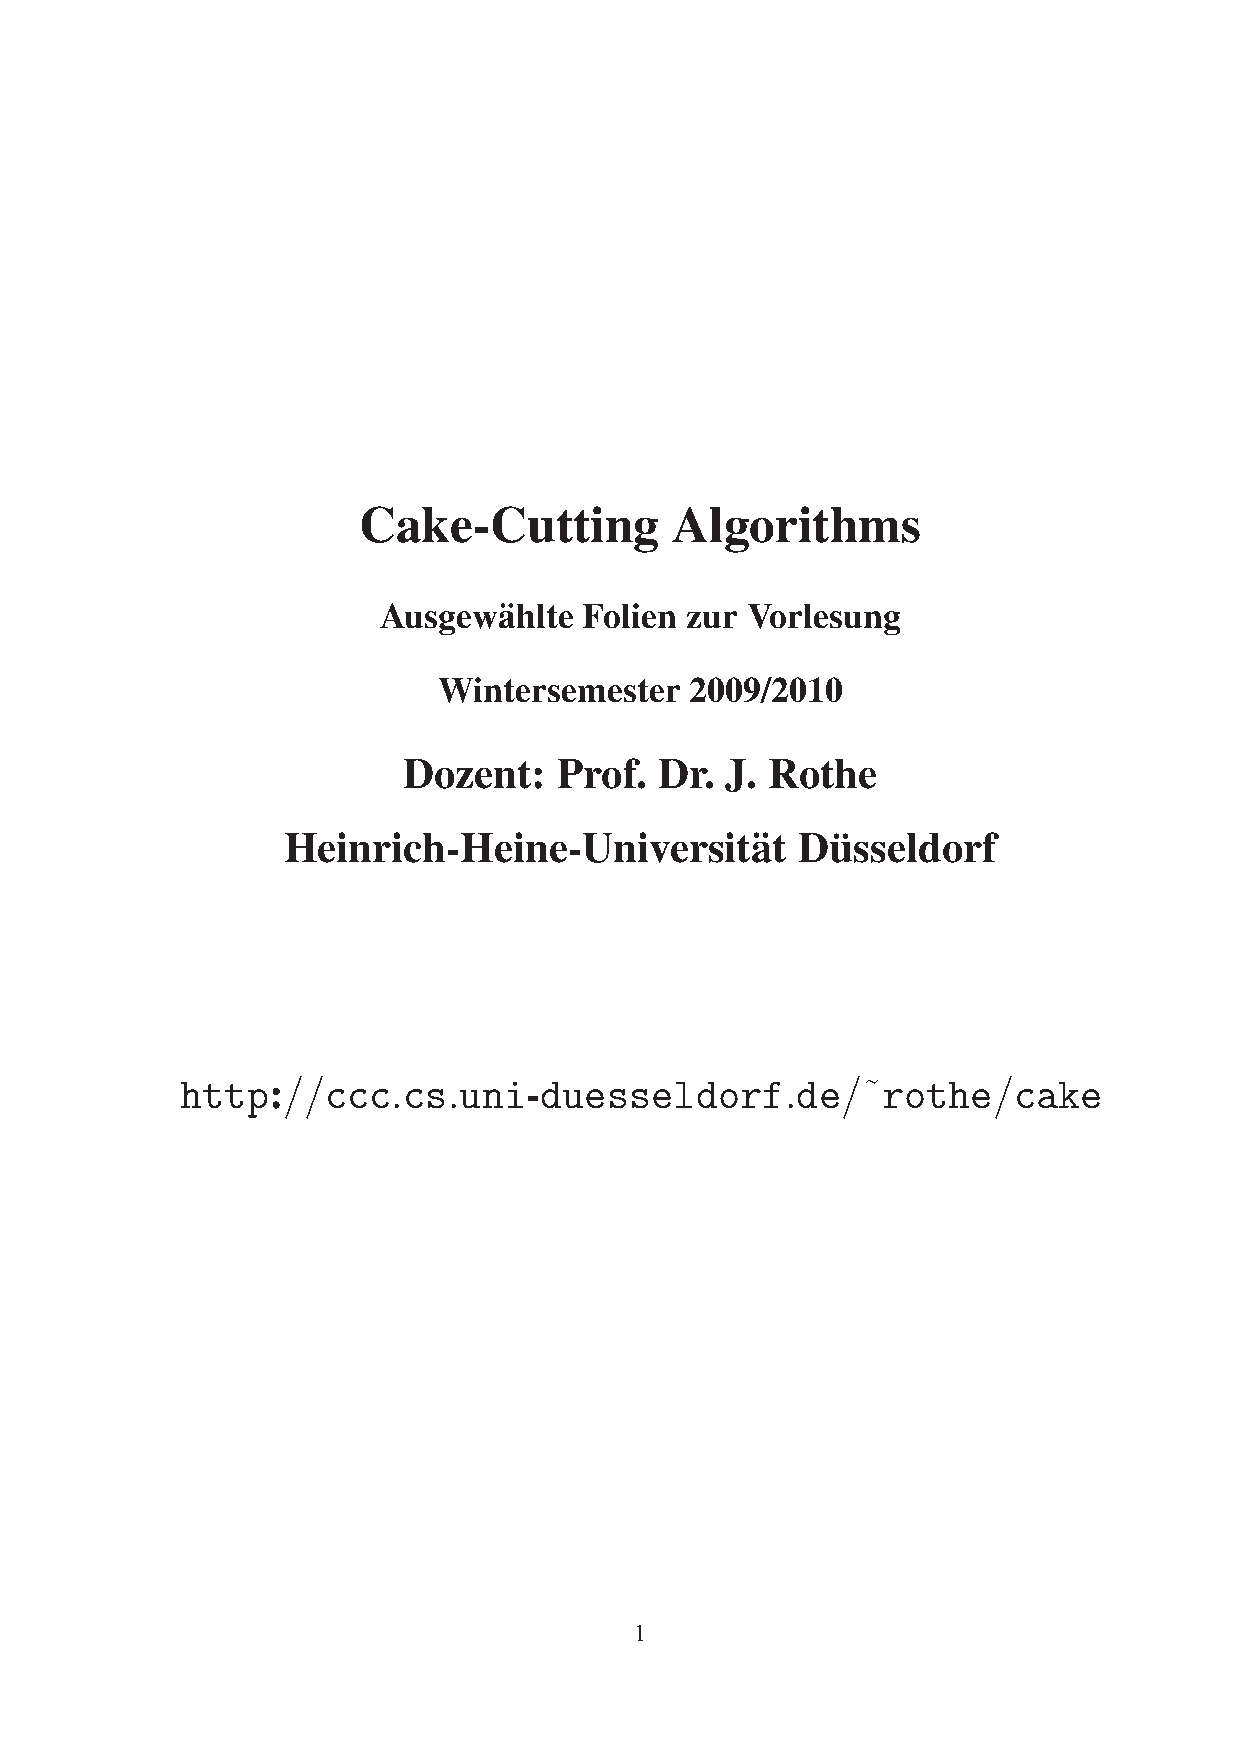
\includepdf[pages=KästchenfolieBis9,scale=0.8]{folien.pdf}
\end{beispiel*}
\includepdf[pages=16,scale=0.8]{folien.pdf}
$\DGEF =$ Anzahl der Neidfrei-Relationen im worst case
\begin{protokoll*}
 Jörg erhält den Kuchen.\\
 $\DGEF: n-1+(n-1)(n-2)=n-1-n^2-3n+2=n^2-2n-1$
\end{protokoll*}
\begin{satz*}
 \begin{enumerate}
  \item Jedes neidfreie CCP für $n\geq1$ Spieler hat einen $\DGEF$ von $n(n-1)$.
  \item Sei $d(n)$ der $\DGEF$ eines proportionalen CCPs mit $n\geq2$ Spielern. Dann gilt: $n\leq d(n)\leq n(n-1)$.
 \end{enumerate}
\end{satz*}
\begin{proof}
 \begin{enumerate}
  \item Da wir $p_i\nVdash p_i$ für alle $i$, $1\leq i\leq n$, außer 8 lassen, hat jeder der $n$ Spieler zu jedem anderen Spieler eine
        Neidfreie-Relation, insgesamt also $n(n-1)$.
  \item \begin{description}
         \item[$n=2$] Offenbar gilt: $d(2)=2$, denn da das CCP proportional ist, gilt: $v_1(X_1)\geq\frac{1}{2}$ und $v_2(X_2)\geq\frac{1}{2}
                    \Rightarrow v_1(X_1)\geq v_1(X_2)$ und $v_2(X_2)\geq v_2(X_1)$
         \item[$n\geq3$] Da $p_i\nVdash p_i$ für alle $i$ ignoriert wird, gilt $d(n)\leq n(n-1)$.
                         \begin{itemize}
                          \item[] In einer proportionalen Aufteilung gilt:\\$v_i(X_i)\geq\frac{1}{n}$ für $1\leq i\leq n$.\\
                          \item[$\Rightarrow$] Keiner der $n$ Spieler kann gleichzeitig alle anderen Spieler bendeidenl, denn:\\
                                               Angenommen, das wäre nicht so. Konkret: $p_1\nVdash p_2$
                          \item[$\Rightarrow$]$v_1(X_2)>v_1(X_1)\geq\frac{1}{n}$
                          \item[$\Rightarrow$]$v_1((X-X_1)-X_2)<\frac{n-2}{n}$
                          \item[$\Rightarrow$]$(X-X_1)-X_2$ kann nicht so in $n-2$ Portionen aufgeteilt werden, dass $v_i(X_j)\geq\frac{1}{n}$
                                              für alle $j,3\leq j\leq n$, gilt.
                          \item[$\Rightarrow$]es gibt ein $j,3\leq j\leq n$, so dass $v_i(X_j)<\frac{1}{n}$, gilt.
                          \item[$\Rightarrow$]$p_i\nVdash p_j$
                         \end{itemize}
                         Also hat jeder der $n$ Spieler mindestens eine garantierte Neidfrei-Relation zu einem anderen Spieler: $n\leq d(n)$  
        \end{description}
 \end{enumerate}
\end{proof}

\begin{lemma}
 Verlangen die Regeln/Strategien eines proportionalen CCPs für $n\geq2$ Spielern von keinem Spieler, die Portionen der anderen Spieler
 zu bewerten, dann ist der $\DGEF=n$.
\end{lemma}
\begin{proof}
 \begin{description}
  \item[$n=2$] Proportionalität $\Rightarrow$ Neidfreiheit\\best case $=$ worst case\\und wie vorher: $\DGEF=2=n$
  \item[$n\geq3$] Betrachte das folgende Szenario: Für eine gegebene Aufteilung $X=\bigcup\limits_{i=1}^nX_i$, die proportional ist, aber sonst
                  keinerlei Einschränkungen unterliegt, setzen wir die Maße der Spieler so: \\Für jedes $i, 1\leq i\leq n$, bewertet $p_i$:
                  \begin{itemize}
                   \item die eigene Portion $X_i$ mit $v_i(X_i)=\frac{1}{n}=\frac{n}{n^2}\Rightarrow$ proportional!
                   \item die Portion $X_j$ eines Spielers $p_j, j\neq i: v_i(X_j)=\frac{2}{n}<\frac{1}{n}$
                   \item jede der $n-2$ übrigen Portionen $X_k$ der Spieler $p_k, |{i,j,k}|=3, v_i=(X_k)=\frac{n+1}{n^2}>\frac{1}{n}$
                  \end{itemize}
                  Insgesamt gilt dann für jedes $i, 1\leq i\leq n$:
                  \begin{enumerate}
                   \item $v_i(X)=v_i(\bigcup\limits_{j=1}^nX_j)\stackrel{\text{Additivität}}{=}\sum\limits_{j=1}^nv_i(X_j)=
                         \frac{1}{n^2}(n+2+(n-2)(n+1))=\frac{1}{n^2}(n+2+n^2+n-2n-2)=1$
                   \item $p_i$ hat $n-2$ Neidrelationen und nur eine Neidfrei-Relation\\$\Rightarrow$ Insgesamt gibt es $n$ garantierte 
                         Neidfrei-Relationen, eine für jeden Spieler.
                  \end{enumerate}
 \end{description}
\end{proof}
\includepdf[pages=17,scale=0.8]{folien.pdf}
\begin{satz}
 Das Last-Diminisher-Protokoll hat einen $\DGEF$ von $\frac{n(n-1)}{2}+2$
\end{satz}
\begin{proof}
 \begin{description}
  \item[Runde 1] Sei $\bar{p}_1$ der Spieler, der die erste Portion erhält. Jeder andere Spieler bewertet diese mit $\leq\frac{1}{n}$,
                 beneidet also $\bar{p}_1$ nicht\\$\Rightarrow n-1$ garantierte Neidfrei-Relationen
  \item[Runde $i, 1<i<n$] Analog zu Runde 1 können $n-i$ Neidfrei-Relationen garantiert werden. $\bar{p}_i$, der die ite Portion erhält, wird
                          von den verbleibenden Spielern nicht beneidet.\\$\Rightarrow$ mindestens $\sum\limits_{i=1}^ni=\frac{n-1}{2}$
                          garantierte Neidfrei-Relationen
  \item[Letzte Runde] \begin{enumerate}
                       \item Cut \& Choose zwischen $\bar{p}_{n-1}$ und $\bar{p}_n$. Keiner dieser beiden beneidet den anderen.\\
                             $\Rightarrow$ eine zusätzliche garantierte Neidfrei-Relation.
                       \item Da Last-Diminisher proportional ist, gibt es eine weitere garantierte Neidfrei-Relation für $\bar{p}_1$
                      \end{enumerate}
 \end{description}
$\Rightarrow\DGEF=\frac{(n-1)n}{2}+2$ 
\end{proof}
\begin{satz}
 Das Lone-Chooser-Protokoll hat einen $\DGEF$ von $n$.
\end{satz}
\begin{proof}
 Kein Spieler bewertet die Portion irgendeines anderen Spielers.\\$\stackrel{\text{Lemma}}{\Longrightarrow}\DGEF=n$
\end{proof}

\section{Gerechte Aufteilung mit einer minimalen Anzahl von Schnitten}
\underline{Motivation}
\begin{itemize}
 \item Effizienz $\widehat{=}$ Faulheit
 \item Ästhetik
\end{itemize}
z.B. Moving-Knife.Protokoll: $n-1$ Schnitte. Besser geht's nicht!\\
$\Rightarrow$ Hier werden keine Moving-Knife-Protokolle, sondern nur endliche Algorithmen betrachtet.
\includepdf[pages=18-19,nup=2x1]{folien.pdf}
\subsection{Grundlegende Annahmen}
\begin{bemerkung*}
 \begin{description}
  \item[1-3] gelten auch für Wahrscheinlichkeitsmaße
  \item[Faltbarkeit] (+Additivität): Jedes Stück kann ohne Wertverlust beliebig oft (endlich!) geteilt werden. 
                                     (Auch: unendliche Additivität)\\
                                     D.h., wenn $v_i(A)=a>0$ und $a_i+a_2=a$, wobei $a_1>0$ und $a_2>0$ beliebig sind, so kann $A$ geteilt
                                     werden in $A=A_1\cup A_2$ mit $v_i(A_1)=a_1, v_i(A_2)=a_2$.
 \end{description}
\end{bemerkung*}
\subsection{Das ``Ein-Schnitt-Genügt''-Protokoll}
Betrachte das Last-Diminsher-Protokoll für 3 Spieler: $C,D,E$
\begin{beispiel}
 $C$ schneidet $S_1$ mit $v_C(S_1)=\frac{1}{N}=\frac{1}{3}\\v_D(S_1)>\frac{1}{3}\Rightarrow$ schneidet was ab und gibt 
 $S_2$ mit $v_D(S_2)=\frac{1}{3}.\\v_E(S_2)<\frac{1}{3}\Rightarrow S_3=S_2$ geht an $D$\\
 $C$ und $E$ spielen Cut \& Choose mit\begin{align}
                                       A = X-S_1\text{ und } B=S_1-S_3
                                      \end{align}
 Müssen diese seperat geteilt werden mit 2 Schnitten ?\\
 Nein! Ein Schnitt genügt.\\
 \underline{im Beispiel:} Angenommen, $v_C(A)=\frac{2}{3}$ und $v_C(B)=\frac{1}{12}$. C soll ein Stück im Wert von 
                          $\frac{1}{2}(\frac{2}{3}+\frac{1}{12})=\frac{9}{24}$\\
 C schneidet $A$ in $A_1$ und $A_2$, so dass \begin{align}
                                              v_C(A_1)=\frac{9}{24}\text{ und }v_C(A_2)=\frac{2}{3}-\frac{9}{24}=\frac{7}{24}
                                             \end{align}
 Es gilt: $v_C(B\cup A_2)=\frac{1}{12}+\frac{7}{24}=\frac{9}{24}$
\end{beispiel}
\begin{satz}
 (Ein-Schnitt-genügt-Prinzip - ESG-Prinzip)\\
Mit einem Schnitt kann ein Spieler $S$, der $X_1,\dots,X_n$ bewertet mit $v_S(X_i)=a_i$, diese im Verhältnis $b:c$ teilen, wobei 
$b+c=a_1+a_2+\dots+a_n$
\end{satz}
\begin{proof}
 Finde das $j$ mit $a_1+a_2+\dots+a_j\leq b<a_{j+1}+\dots+a_n$ und schneide $X_{j+1}$(mit Wert $a_{j+1}$ in $X'_{j+1}$ und $X''_{j+1}$
 mit \begin{align*}
      v_S(X'_{j+1})=b-(a_1+\dots+a_j)\\
      v_S(X''_{j+1})=a_{j+1}-v_S(X'_{j+1})
     \end{align*}
 Dann gilt für $A=X_1\cup X_2\cup\dots\cup X_j\cup X'_{j+1}$ und für $B=X''_{j+1}\cup X_{j+2}\cup\dots\cup  X_n$:
 \begin{align*}
  v_S(A)=a_1+a_2+\dots+a_j+b-(a_1+\dots+a_j)=b\\
  v_S(B)=a_{j+1}-b+a_1+\dots+a_j+a_{j+2}+\dots+a_n=a_1+a_2+\dots+a_n-b=c
 \end{align*}
\end{proof}
\begin{beispiel*}
 ESG-Prinzip\\
 Angenommen, für Spieler $S$ haben die Stücke $X_1,X_2,\dots,X_5$ die Werte:
 \begin{align*}
  v_S(X_1)=0.15, v_S(X_2)=0.2, v_S(X_3)=0.1, v_S(X_4)=0.25, v_S(X_5)=0.1, \text{insgesamt } 0.8
 \end{align*}
 und $S$ soll sie im Verhältnis $3:5$ teilen, soll also $A$ und $B$ finden mit
 \begin{eqnarray*}
  &v_S(A)=0.3\text{ und }v_S(B)=0.5\\
  &\Rightarrow j=1: 0.15\leq0.3<0.15+0.2=0.35\\
  &\Rightarrow S\text{ schneidet }X_2\text{ in }X'_2\text{ und }X''_2\text{ mit }v_S(X'_2)=0.15\text{ und }v_S(X''_2)=0.05\\
  &\Rightarrow A=X_1\cup X'_2\text{ hat Wert }0.3, B=X''_2\cup X_3\cup X_4\cup X_5\text{ hat Wert }0.5\\
 \end{eqnarray*}
\end{beispiel*}
\subsection{Erforderliche Anzahl von Schnitten für einige CCPs}
Aussage: ``Protokoll $\Pi$ erfordert $k$ Schnitte'' heißt:
\begin{enumerate}
 \item $\Pi$ kann mit $\leq k$ Schnitten ausgeführt werden
 \item $\Pi$ benötigt im worst case $\geq k$ Schnitte
\end{enumerate}
\begin{fakt}
 Das Last-Diminisher-Protokoll erfordert für $n\geq2$ Spieler
 \begin{align*}
  \frac{n^2+n-4}{2}\text{ Schnitte}
 \end{align*}
\end{fakt}
\begin{proof}
 Es gibt $n-1$ Runden\\
 In Runde $i, 1\leq i\leq n-2$, schneidet (oder markiert) jeder der $n-i+1$ beteiligten Spieler.\\
 In Runde $n-1$ genügt nach dem ESG 1 Schnitt\\
 $\Rightarrow$ insgesamt $(\sum\limits_{i=1}^{n-2}n-i+1)+1=n+(n-1)+\dots+3+1=\frac{n(n+1)}{2}-2=\frac{n^2+n-4}{2}$
\end{proof}
\includepdf[pages=20,scale=0.8]{folien.pdf}
\begin{fakt}
 Das Modified Last-Dimisher-Protokoll erfordert
 \begin{align*}
  \frac{n(n-1)}{2}\text{ Schnitte}
 \end{align*}
\end{fakt}
\begin{proof}
 Wie oben, aber 1 Schnitt pro Runde $i\leq n-2$ weniger:
 \begin{align*}
  \sum\limits_{i=1}^{n-1}n-i=(n-1)+(n-2)+\dots+1=\frac{n(n-1)}{2}
 \end{align*}
\end{proof}
\begin{beispiel*}
 $n=100: 4950$ Schnitte
\end{beispiel*}
\includepdf[pages=21,scale=0.8]{folien.pdf}
\subsubsection{Analyse vom Lone-Chooser-Protokoll ohne ESG-Prinzip}
Wenn in der $(n-1)$-ten Runde $p_n$ hinzukommt:
\begin{itemize}
 \item hat jeder von $p_1,\dots,p_{n-1}$ bereits $(n-2)!$ Stücke
 \item teilt diese in $n$ Teilstücke
\end{itemize}
 \begin{tabular}{ccccccc}$\Rightarrow$&$(n-2)!$&$\cdot$&$(n-1)$&$\cdot$&$n$&$=n!$\\
            &\#Stücke zu Beginn&&\#bisheriger Spieler&&\#der Teilstücke,&\\
              &von Runde n-1 &&&&die jeder&\\
              &&&&&bisherige Spieler&\\
              &&&&&für jedes&\\
              &&&&&bisherige Stück&\\
              &&&&&erzeugt&
               \end{tabular}\\
Stücke erfordern $n!-1$ Schnitte.
\subsubsection{Analyse vom Lone-Chooser-Protokoll mit ESG-Prinzip}
\begin{description}
 \item[$n=2$] 1 Schnitt
 \item[$n=3$] 2 Cutter teilen ihr Stück mit je 2 Schnitten\\$\Rightarrow 1+2\cdot2=5$ Schnitte insgesamt
 \item[$n=4$] 3 Cutter teilen je 2 Stücke und sollen 4 Stücke erzeugen. Statt $3\cdot2$ Schnitte pro Cutter (insgesamt 18) genügen nach
              dem ESG 3 Schnitte pro Cutter
 \item[$n=5$] analog zu $4\cdot4$ Schnitten\\$\Rightarrow\sum\limits_{i=1}^{n-1}i^2=\frac{(n-1)n(2n-1)}{6}\in \mathcal{O}(n^3)
              \text{ immer noch schneller als } \mathcal{O}(n^2)$
\end{description}
Can we do better?
\begin{center}
 \includegraphics[height=0.35\textheight]{fig/obama_ywc.png}
\end{center}
\subsection{Der Divide \& Conquer Algorithmus}
Last-Diminisher: nach dem $n$-ten Schnitt ist 1 Spieler happy und $n-1$ Spieler can be made happy.
\begin{idee}
 Aufteilung in 2 Spielergruppen von etwa gleicher Größe $\sim \frac{n}{2}$, die jeweils einen Teil des Kuchens unter sich aufteilen.
\end{idee}
\begin{protokoll*}
 \underline{Divide \& Conquer} (Even \& Paz, 1984)\\
 Hilfreich sind die einfachen Fälle:
 \begin{description}
  \item[$n=1$] kein Schnitt nötig
  \item[$n=2$] Nach ESG genügt 1 Schnitt
  \item[$n=3$] Modified Last-Diminisher-Protokoll: 3 Schnitte
 \end{description}
 Nicht einfache Fälle:
 \begin{description}
  \item[$n=4$] $p_1,p_2,p_3$ halbieren den Kuchen jeweils nach ihrem Maß mit parallelen Schnitten.
               \begin{center}
                \includegraphics[height=0.2\textheight]{fig/DivideConquerKuchen01}
               \end{center}
               $p_4$(Non-Cutter) bewertet die durch den Mittelschnitt definierten Stücke $A$ und $X-A$.\\
               Sei $v_4(A)\geq v_4(X-A)$. Dann teilen jeweils mit Cut \& Choose
               \begin{itemize}
                \item $p_3$(der Spieler mit dem ``linkesten'' Schnitt) und $p_4$ das Stück $A$
                \item $p_1$ und $p_2$(die beiden übrigen Spieler) teilen sich den Rest $X-A$
               \end{itemize}          
               \begin{bemerkung*}
               $v_2(A)=v_2(X-A)$, also ist es $p_2$(der den Mittelschnitt tat) egal, ob er $A$ oder $X-A$ teilt
               \end{bemerkung*}
               $\Rightarrow$ Insgesamt: $3+1+1=5$ Schnitte
  \item[$n=5$] $p_1,p_2,p_3,p_4$ machen parallele Schnitte im Verhältnis $2:3$ nach ihrem Maß
               \begin{center}
                \includegraphics[height=0.2\textheight]{fig/DivideConquerKuchen02}
               \end{center}
               $p_5$(Non-Cutter) bewertet $A$ und $X-A$.
               \begin{itemize}
                \item Ist $v_5(A)\geq\frac{2}{5}$, so teilen\\$p_4\&p_5 A$ mit Cut \& Choose und \\
                      $p_1,p_2,p_3 X-A$ mit Modified Last-Diminisher.
                \item Ist $v_5(X-A)\geq\frac{3}{5}$, so teilen\\$p_2,p_3,p_5$ das Stück $X-A$ mit Modified Last-Diminisher\\
                      $p_1\&p_4$ das Stück $A$ mit Cut \& Choose 
               \end{itemize}
               \begin{bemerkung*}
                \begin{enumerate}
                 \item Gilt $v_5(A)=\frac{2}{5}\text{ und }v_5(X-A)=\frac{3}{5}$, so ist $p_5$ egal, ob er $A$ oder $X-A$ teilt
                 \item Genauso für den Spieler mit dem Mittelschnitt($p_1$)
                \end{enumerate}
               \end{bemerkung*}
               Insgesamt: $4+3+1=8$ Schnitte
 \end{description}
\end{protokoll*}
\includepdf[pages=22-23,nup=2x1]{folien.pdf}
Bezeichnet man mit $D(n)$ die Zahl der Schnitte, die Divide \& Conquer für eine faire (prop.) Aufteilung für $n$ Spieler erfordert, so gilt:
\begin{eqnarray*}
 D(2k) &=& 2k-1+2D(k), k\geq2\\
 D(2k+1) &=& 2k+D(k)+D(k+1), k\geq2\\
 D(1) &=& 0\\
 D(2) &=& 1\\
 D(3) &=& 3 \\
 D(n) &=& (n-1)+D(\left\lfloor\frac{n}{2}\right\rfloor)+D(\left\lceil\frac{n}{2}\right\rceil)
\end{eqnarray*}
\begin{satz*}
 $D(n)\stackrel{\smiley}{=}n\cdot k-2^k+1$, wobei $k=\lceil\log n\rceil$\\
 Grob gesprochen: $\mathcal{O}(n\log n)$ Schnitte reichen.
\end{satz*}
\begin{proof}
 Induktion über $n$:
 \begin{description}
  \item[IA] \begin{description}
             \item[$n=1$] $n\cdot k-2^k+1=1\cdot0-2^0+1=0-1+1=0=D(1)\checkmark$
             \item[$n=2$] $D(2)=1+2D(1)=1+2\cdot0=1\checkmark$ 
            \end{description}
  \item[IV] Sei $n>2$ und Beh. seit richtig für $1,2,\cdots,n-1$.\\
            Für $k=\lceil\log n\rceil$ sei $n=2^{k-1}+r$ mit $1\leq r\leq2^{k-1}$\\
            Da $n>2$ und $r\leq2^{k-1}$, gilt $2^{k-1}>1$, also $k>1$
  \item[IS] \begin{description}
             \item[Fall 1] $r=2\cdot s$ (also gerade) für ein s, $1\leq s\leq2^{k-2}$
                            \begin{eqnarray*}
                             \Rightarrow D(n)&\stackrel{\smiley}{=}&(n-1)+2D\left(\frac{n}{2}\right)\text{, denn } n=2^{k-1}+r
			      \text{ ist gerade wegen }k>1\\
                             &\stackrel{IV}{=}&(2^{k-1}+2s-1)+2[(2^{k-2}+s)\lceil\log(2^{k-1}+s)\rceil-2^{\lceil\log(2^{k-2})+s\rceil}+1]\\
                             &=&(2^{k-1}+2s-1)+2[(2^{k-2}+s)(k-1)-2^{k-1}+1]\\
                             &=&2^{k-1}(k-2)+2sk+1\\
                             &=&(2^{k-1}+2s)k-2^k+1=nk+2^k+1\checkmark
                            \end{eqnarray*}
                            mit
                            \begin{eqnarray*}
                             2^k<2^{k-2}+s\leq2\cdot2^{k-2}=2^{k-1}\\
                             \Rightarrow\lceil\log(2^{k-2}+s)\rceil=k-1
                            \end{eqnarray*}
             \item[Fall 2] $r=2s+1$ (also ungerade) für ein $s, 0\leq s\leq2^{k-2}-1$\\Sei $s\neq0$
                           \begin{eqnarray*}
                            D(n)&\stackrel{\smiley}{=}&(2^{k-1}+2s)+D(2^{k-2}+s+1)+D(2^{k-2}+s)\\
                            &\stackrel{IV}{=}&(2^{k-1}+2s+[(2^{k-2}+s+1)\lceil\log(2^{k-2}+s+1)\rceil-2^{\lceil\log(2^{k-2}+s+1)\rceil}+1]\\
                            && +[(2^{k-2}+s)\lceil\log(2^{k-2}+s)\rceil-2^{\lceil\log(2^{k-2}+s)\rceil}+1]\\
                            &=&(2^{k-1}+2s)+[(2^{k-2}+s+1)(k-1)-2^{k-1}+1]\\
                            && +[(2^{k-2}+s{\color{green}+1})(k-1)-2^{k-1}+1]\color{green}-(k-1)\\
                            &=&(2^{k-1}+2s)+2[(2^{k-2}+s+1)(k-1)-2^{k-1}+1]\color{green}-(k-1)\\
                            &=&(2^{k-1}+2s+1)+(2^{k-1}+2s+2)(k1)-2^k+1\color{green}-(k-1)\\
                            &=&(2^{k-1}+2s+1)+(2^{k-1}+2s+{\color{green}1})(k-1){\color{green}}+(k-1)-2^k+1\color{green}-(k-1)\\
                            &=&(2^{k-1}+2s+1)k-2^k+1=n\cdot k-2^k+1\checkmark
                           \end{eqnarray*}
                           mit
                           \begin{eqnarray*}
                            2^{k-2}+1\stackrel{s\neq0}{<}2^{k-2}+s+1\stackrel{s\leq2^{k-2}-1}{\leq}2\cdot2^{k-2}=2^{k-1}\\
                            \Rightarrow \lceil\log(2^{k-2}+s+1)\rceil=\lceil\log(2^{k-2}+s)\rceil=k-1
                           \end{eqnarray*}
                           Ist $s=0$, so ergibt sich oben: $\lceil\log(2^{k-2}+s)\rceil=k\cdot2$ und man erhält:
                           $D(n)=(2^{k-1}+1)k+2^k+1=n\cdot k-2^k+1$\checkmark
            \end{description}
 \end{description}
\end{proof}
\begin{bemerkung*}
 Divide \& Conquer ist proportional und endlich beschränkt.
\end{bemerkung*}
\includepdf[pages=24,scale=0.8]{folien.pdf}
\includepdf[pages=25,scale=0.8]{folien.pdf}
\subsection{Zwei Schnitte reichen nicht für drei Spieler}
Moving Knife: 2 Schnitte!
\begin{fakt}
 Das Viertel-Protokoll für Drei garantiert jedem der 3 Spieler mit 2 Schnitten $\geq\frac{1}{4}$ des Kuchens. $\square$
\end{fakt}
\begin{satz*}
 Kein endliches CCP kann 3 Spielern mit 2 Schnitten einen proportionalen Anteil garantieren, sondern höchstens $\frac{1}{4}$ des Kuchens.
\end{satz*}
\begin{proof}
 Sei $p_1$ der Spieler, der den ersten Schnitt macht:
 \begin{align*}X=X_1\cup X_2\end{align*}
 Da $p_2, p_3$ keine Kontrolle über den Schnitt haben, ist es möglich, dass $v_2(X_1)=v_3(X_1)=\frac{1}{2}=v_2(X_2)=v_3(X_2)$\\
 O.B.d.A. sei $v_1(X_1)\geq\frac{1}{2}$
 \begin{description}
  \item[Fall 1] $p_1$ schneidet $X_1$ oder $X_2$ in 2 Stücke.\\
                Egal welches, kann wegen $v_2(X_2)=v_3(X_2)=\frac{1}{2}$ passieren, dass sowohl $p_2$ als auch $p_3$, die neuen Stücke
                jeweils mit $\frac{1}{4}$ bewerten.\\
                $\Rightarrow$ wenigstens einer von $p_2$ oder $p_3$ muss ein solches Stück nehmen, also nur $\frac{1}{4}$ des Kuchens erhalten.
  \item[Fall 2] $p_2$ oder $p_3$ (sagen wir: $p_2$) macht den 2. Schnitt.\\
                Wegen $v_2(X_1)=v_2(X_2)=\frac{1}{2}$\\
                $\Rightarrow p_2$ bewertet eines der neuen Stücke mit $\leq\frac{1}{4}$\\
                Da $p_1 \& p_3$ haben keine Kontrolle über den 2. Schnitt\\
                $\Rightarrow$ möglich: sie bewerten dieses Stück ebenfalls mit $\leq\frac{1}{4}$\\
                $Rightarrow$ einer von $p_1,p_2,p_3$ muss es nehmen
 \end{description}
\end{proof}
\subsection{Vier Schnitte für vier Spieler}
\begin{idee}
 Angenommen, $X=A\cup B\cup C\cup D$ und\begin{eqnarray*}
                                        &v_1(A)\geq v_1(B)\text{ und }v_1(C)\geq v_1(D)\\
                                        &\Rightarrow v_1(A\cup C)\geq\frac{1}{2}
                                        \end{eqnarray*}
 $p_1$ wäre also bereit, $A\cup C$ mit irgendwem mit Cut \& Choose zu teilen.\\
 \underline{Sprechweise:} Für Spieler $p_i$ und Stücke $A$ und $B$ sagen wir:
 \begin{itemize}
  \item $p_i$ \underline{bevorzugt $A$ über $B$}, falls $v_i(A)\geq v_i(B)$
  \item $p_i$ \underline{bevorzugt $A$ echt über $B$}, falls $v_i(A)>v_i(B)$
  \item für $p_i$ ist $A$ \underline{akzeptabel}, falls $v_i(A)\geq\frac{1}{n}$, wobei $n$ die Anzahl der Spieler ist.
 \end{itemize}
\end{idee}
\subsubsection*{Viertel-Protokoll für Vier}(Even \& Paz, 1984)\\
 \underline{Gegeben:} Spieler $p_1,p_2,p_3,p_4$ Kuchen $X$\\
 $p_1$ teilt $X=Y\cup Z$ mit $v_1(Y)=v_1(Z)=\frac{1}{2}$
 \begin{description}
  \item[Fall 1] $p_2,p_3,p_4$ bevorzugen nicht alle dasselbe Stück (über das andere).\\
                Wir dürfen annehmen: $v_2(Y)\geq\frac{1}{2},v_3(Y)\geq\frac{1}{2},v_4(Z)\geq\frac{1}{2}$.
                \begin{itemize}
                 \item $p_2\&p_3$ teilen $Y$ mit Cut \& Choose und erhalten akzeptable Stücke
                 \item $p_1\&p_4$ teilen $Z$ mit Cut \& Choose und erhalten akzeptable Stücke
                \end{itemize}
                3 Schnitte waren genug.
  \item[Fall 2] $p_2,p_3,p_4$ bevorzugen echt dasselbe Stück.\\
                Wir nehmen an: $v_i(Z)>\frac{1}{2}$ für alle $i\in{2,3,4}$
                \begin{itemize}
                 \item $p_1$ teilt $Y=Y_1\cup Y_2$, so dass $v_1(Y_1)=v_1(Y_2)=\frac{1}{4}$.
                       \begin{description}
                        \item[Fall 2.1] Auch wenn $v_i(Y)<\frac{1}{2}$ für $i\in{2,3,4}$ könnte einer von $p_2,p_3,p_4$ ein $Y_i$ akzeptabel
                                        finden sagen wir: $p_2$\\Dann sind wir wieder mit 3 Schnitten fertig:
                                        \begin{itemize}
                                         \item $p_2$ erhält $Y_i$
                                         \item $p_1$ erhält das ander $Y_j$
                                         \item $p_3\&p_4$ teilen $Z$ mit Cut \& Choose und erhalten $>\frac{1}{4}$
                                        \end{itemize}
                        \item[Fall 2.2] Keiner von $p_2,p_3,p_4$ hält $Y_1$ oder $Y_2$ für akzeptabel. Trotzdem bevorzugt jeder eines dieser
                                        Stücke.\\$\Rightarrow$ Zwei von $p_2,p_3,p_4$ müssen dasselbe Stück bevorzugen.
                                        \begin{description}
                                         \item[Annahme:] $p_2,p_3$ bevorzugen $Y_2$.\\$\Rightarrow v_i(Y_2)\geq v_i(Y_1)$ für $i\in{2,3}$\\
                                                         (Welches $Y$-Stück $p_4$ bevorzugt ist egal.) 
                                        \end{description}
                                        \begin{itemize}
                                         \item $p_1$ erhält $Y_1$ und scheidet aus.
                                        \end{itemize}
                                        \begin{bemerkung*}
                                         $p_2,p_3,p_4$ teilen $X-Y_1=Y_2\cup Z$.\\Erfordert das nicht 3 Schnitte, insgesamt also 5? Nein!
                                        \end{bemerkung*}
                                        \begin{itemize}
                                         \item $p_2$ teilt $Z=Z_1\cup Z_2$ mit $v_2(Z_1)=v_2(Z_2)>\frac{1}{4}$
                                         \item \underline{Wir wissen bereits:}\\
                                               \begin{tabular}{c|cccc}
                                                 &$Y_1$&$Y_2$&$Z_1$&$Z_2$\\ \hline
                                                 $p_2$ & - &*-&*+&*+\\
                                                 $p_3$ & -&*-&&\\
                                                 $p_4$ &-&-&&
                                               \end{tabular}
                                               \begin{tabular}{cl}
                                                Legende: &+ akzeptabel\\
                                                &- inakzeptabel\\
                                                &* bevorzugt\\
                                                &$(Y_1\text{ vs. }Y_2\text{ | }Z_1\text{ vs. }Z_2)$
                                               \end{tabular}

                                        \end{itemize}
                                        Und die anderen 4 Einträge ?\\
                                        Wenn $p_3$ oder $p_4$ ein $Z$-Stück bevorzugt, dann ist es für ihn akzeptabel, wegen $v_i(Z)>\frac{1}{2}
                                        $ für $i\in{3,4}$.\\
                                        Wir dürfen annehmen: $p_3$ bevorzugt $Z_1$.
                                        \begin{enumerate}
                                         \item[a)] $p_4$ findet $Z_2$ akzeptabel. Dann gilt:\\
                                               \begin{tabular}{c|cc}
                                                &$Z_1$&$Z_2$\\\hline
                                                $p_3$&*+&\\
                                                $p_4$&&+
                                               \end{tabular}
                                               \begin{itemize}
                                                \item Dann erhält $p_4$ das Stück $Z_2$
                                                \item $p_2\&p_3$ teilen $Y_2\cup Z_1$ mit Cut \& Choose, denn nach Herrn Schulenbergs Idee ist
                                                      \begin{eqnarray*}
                                                       v_i(Y_2\cup Z_1)\geq\frac{1}{2}\text{ für }i\in{2,3}
                                                      \end{eqnarray*}
                                               \end{itemize}
                                               $\Rightarrow$ alle Spieler sind zufrieden nach 4 Schnitten.
                                         \item[b)] $Z_2$ ist für $p_4$ inakzeptabel. Dann gilt:\\
                                                  \begin{tabular}{c|cc}
                                                   &$Z_1$&$Z_2$\\\hline
                                                   $p_3$&*+&\\
                                                   $p_4$&&-
                                                  \end{tabular}
                                                  \begin{itemize}
                                                   \item $p_2$ erhält $Z_2$
                                                   \item $p_3\&p_4$ teilen $Y_2\cup Z_1$ mit Cut \& Choose.\\
                                                         Da $p_3$ beide Stücke ($Y_2\&Z_1$) bevorzugt, gilt
                                                         \begin{eqnarray*}
                                                          v_3(Y_2\cup Z_1)\geq\frac{1}{2}
                                                         \end{eqnarray*}
                                                         Da $p_4$ bereits zwei inakzeptable Stücke ($Y_1\&Z_2$) abgelehnt hat, gilt $v_4(Y_2\cup
                                                         Z_1)\geq\frac{1}{2}$
                                                  \end{itemize}
                                                  $\Rightarrow$ alle sind zufrieden nach 4 Schnitten
                                        \end{enumerate} 
                       \end{description}
                \end{itemize}$\square$
 \end{description} 
\begin{satz*}
 Das Viertel-Protokoll für Vier garantiert jedem der 4 Spieler einen proportionalen Anteil. (Even \& Paz, 1984)
\end{satz*}
Das ist optimal.
\begin{satz*}
 Kein endliches CCP kann 4 Spielern mit 3 Schnitten einen Anteil von mehr als $\frac{1}{6}$ garantieren (insbesondere nicht $\frac{1}{4}$).
 $\square$
\end{satz*}
\subsection{Verallgemeinerungen}
\subsubsection{Minimale Schnittzahl, um einen proprtionalen Anteil zu garantieren}
\underline{Erinnerung:} Nur endliche Protokolle!
\begin{align*}
 F(1)=0, F(2)=1, F(3)=2, F(4)=4
\end{align*}
Da $F(n)\leq D(n)$ für alle $n$ und $D(n)\in\mathcal{O}(n\log n)$, folgt $F(n)\in\mathcal{O}(n\log n)$\\
Da $F(4)=4<5=D(4)$, geht's für kleine $n$ besser.\\
Divide \& Conquer teilt Spieler in $2\approx$ gleichgroße Gruppen\\
$\Rightarrow \smiley D(n)=(n-1)+D(\lfloor\frac{n}{2}\rfloor)+D(\lceil\frac{n}{2}\rceil)$
\includepdf[pages=26,scale=0.8]{folien.pdf}
Neuer Ansatz (Robertson \& Webb):\\
\begin{tabular}{rll}
 Statt im Verhältnis & $k:k$&für $n=2k$\\
 bzw. &$k:k+1$& für $n=2k+1$
\end{tabular}\\
teilen wir im Verhältnis $t:n-t$ mit $n-1$ Schnitten.\\
$\Rightarrow$ neue Rekurrenz für obere Schranke $E$ von $F$ (d.h. $F(n)\leq E(n)$ für alle $n$):
\begin{align*}
 E(n)=(n-1)+E(t)+E(n-t)
\end{align*}
Man kann zeigen: $E(n)\leq n\log n-1.12n\text{, für }n\geq 8$:
\begin{itemize}
 \item Durch Ausrechnen für $8\leq n\leq15$
 \item Mit Induktion:\\ Gilt $E(n)\leq n\log n-c\cdot n$ für festes $c$ und alle $n$ mit $t\leq n\leq2t-1$, dann gilt obige Umgleichung
       für alle $n\geq8$
\end{itemize}
Welche unteren Schranken gelten?
\begin{satz*}
 (Edmonds \& Pruhs, 2006): $F(n)\in\Omega(n\log n)$.\\
Dies verbessert die $\Omega(n\log n)$-Scranke von Woeginger \& Sgall, die nur für ``zusammenhängende'' proportionale CCPs gilt.
\end{satz*}
\begin{satz*}
 (Procaccia, 2009): Jedes neidfreie endliche CCP erfordert $\Omega(n^2)$ Schnitte
\end{satz*}
Offen: obere Schranke für $n\geq4$.
\begin{center}\includegraphics[height=0.2\textheight]{fig/frog.png}\end{center}
\subsubsection{Was kann $n$ Spielern mit $k$ Schnitten garantiert werden?}
\underline{Wissen:} $M(2,1)=\frac{1}{2}$, $M(3,3)=\frac{1}{3}$, $M(4,4)=\frac{1}{4}$, $M(3,2)=\frac{1}{4}$, $M(4,3)=\frac{1}{6}$\\
Man kann zeigen: $M(5,4)=\frac{1}{8}$, $M(5,5)=\frac{1}{6}$, $M(5,6)=\frac{1}{5}$\\
Gilt $M(n,k_0)=\frac{1}{n}$ für $k_0$, dann gilt $M(n,k)=\frac{1}{n}$, für alle $k\geq k_0$.
\begin{satz*}\item[]
 \begin{enumerate}
  \item $M(n,n-1)=\frac{1}{2n-2}$, für alle $n\geq2$.
  \item $M(n,n)=\frac{1}{2n-4}$ für alle $n\geq4$ und $M(3,3)=\frac{1}{3}$.
  \item $M(n,n+1)\leq\frac{1}{2n-5}$ für alle $n\geq5$.
 \end{enumerate}
\end{satz*}
\includepdf[pages=27,scale=0.8]{folien.pdf}
\subsubsection{Ungleiche Anteile}
Angenommen, $C$ \& $D$ wollen den Kuchen im Verhälntnis $7:4$ teilen.
\begin{idee}
 \begin{enumerate}\item[]
  \item Klone $C$ in $7$ Spielerinnen und $D$ in $4$ Spielerinnen und wende ein bekanntes Protokoll für gleiche Anteile (z.B. Divide \&
        Conquer) auf diese $11$ Spielerinnen an. $C$ und $D$ erhalten alle Anteile ihrer Klone.
        \begin{bemerkung*}
         Klappte für Verhältnisse $r:s$ mit rationalen $r$ und $s$. Schwieriger für irrationale Werte, z.B.: $\pi:13$
        \end{bemerkung*}
        \textbf{Nachteil} Klonen treibt die Schnittzahl hoch.\\
        Im Bsp: $D(11)=10+D(5)+D(6)=10+8+(5+2D(3))=18+11=29$
  \item \underline{Cut-Ones-Algorithmus}
        \begin{itemize}
         \item $C$ teilt $X$ in $11$ Stücke gleichen Werts, also im Verhältnis $1:1:\cdots:1$
         \item $D$ wählt die, nach ihrem Maß, $4$ besten Stücke aus
         \item $C$ erhält die übrigen $7$ Stücke, also $\frac{7}{11}$ des Kuchens
        \end{itemize}
        Klar: $D$ erhält $\geq\frac{4}{11}$, selbst wenn einzelne ihrer $4$ Stücke $<\frac{1}{11}$ wert sind.\\
        Nur 10 Schnitte nötig (deutlich besser als Divide \& Conquer).\\
        Verbesserungen sind möglich: ``Ramsey-Theorie''!
 \end{enumerate}
\end{idee}

\section{Das Lone-Divider-Protokoll}
\subsection{Steinhaus' Lone-Divider-Methode für 3 Spieler}
Seien $C$, $D$, $E$ die Spieler.
\begin{enumerate}
 \item $C$ teilt $X=X_1\cup X_2\cup X_3$ mit $v_C(X_1)=v_C(X_2)=v_C(X_3)=\frac{1}{3}$
 \item $D$ \& $E$ markieren die für sie akzeptablen Stücke.\\
       $X_i$ ist für $D$ akzeptable, falls $v_D(X_i)\geq\frac{1}{3}$.
       \begin{bemerkung*}
        Für beide ist mindestens ein $X_i$ akzeptabel.
       \end{bemerkung*}
 \item \begin{description}
        \item[Fall 1] Für $D$ oder $E$ (sagen wir: $D$) sind sogar 2 der $X_i$ akzeptabel. Dann wählen sie in der Reihenfolge: $E$, $D$, $C$
                      und erhalten alle akzeptable Stücke.
        \item[Fall 2] $D$ und $E$ finden höchstens eins (genau eins) der Stücke $X_1$, $X_2$, $X_3$ akzetabel.
                      \begin{description}
                       \item[2.1] Sind dies verschiedene Stücke, so erhalten $D$ \& $E$ jeweils ihr akzeptables Stück, $C$ das letzte.
                       \item[2.2] Ist dies dasselbe Stück (sagen wir: $X_1$), dann sind $X_2$ \& $X_3$ inakzeptabel für $D$ \& $E$.\\
                                  $C$ erhält $X_3$.\\
                                  $\Rightarrow X'=X-X_3=X_1\cup X_2$ ist dann für $D$ \& $E$ $>\frac{2}{3}$ wert, sie teilen es mit
                                  Cut \& Choose und erhalten $>\frac{2}{3}\cdot\frac{1}{2}=\frac{1}{3}$ von $X$.
                      \end{description}
       \end{description}
\end{enumerate}
\subsection{Custers Lone-Divider-Methode für 4 Spieler}
Seien $C$, $D$, $E$ und $F$ die Spieler.
\begin{enumerate}
 \item $C$ teilt $X=X_1\cup X_2\cup X_3\cup X_4$ mit $v_C(X_1)=v_C(X_2)=v_C(X_3)=v_C(X_4)=\frac{1}{4}$
 \item $D$, $E$ und $F$ markieren ihre akzeptablen Stücke (im Wert von $\geq\frac{1}{4}$)
 \item Betrachte 3 Fälle
       \begin{description}
        \item[Fall 1] Mindestens eines der $X_i$ ist \emph{nur} für $C$ akzeptabel.
         \begin{itemize}
          \item $C$ erhält dieses.
          \item $D$, $E$, $F$ teilen den Rest (im Wert von $>\frac{3}{4}$) mit Steinhaus' Lone-Divider für 3 Spieler und erhalten alle
                $>\frac{3}{4}\cdot\frac{1}{3}=\frac{1}{4}$
         \end{itemize}
         \item[Fall 2] Mindestens ein $X_i$ (sagen wir: $X_1$) ist \emph{nur} für $C$ und eine weitere Spielerin (sagen wir: $D$) akzeptabel.
          \begin{itemize}
           \item $D$ erhält $X_1$
           \item $C$, $E$, $F$ teilen den Rest $X'=X_2\cup X_3\cup X_4$ mit Steinhaus' Lone-Divider-Methode für 3 Spieler und erhalten wegen 
                 $v_C(X')=\frac{3}{4}$ und $v_E(X')>\frac{3}{4}$ und $v_F(X')>\frac{3}{4}$ alle eine akzeptable Portion.
          \end{itemize}
          \item[Fall 3] Weder Fall 1 noch Fall 2.\\
                        D.h. für jedes $i$, $1\leq i\leq4$, ist $X_i$ für $C$ und mindestens zwei weitere Spieler akzeptabel.\\
                        \begin{tabular}{cccc}
                         $X_1$ & $X_2$ & $X_3$ & $X_4$\\\hline
                         C&C&C&C\\
                         ?&?&?&?\\
                         ?&?&?&?\\
                        \end{tabular}
                        $\left\{\begin{tabular}{l}Spieler, für die\\die $X_i$ akzeptabel\\sind.\end{tabular}\right\}$\\
                        Wenn keiner von $D$, $E$, $F$ mindestens drei der $X_i$ akzeptabel findet, dann könnten wir höchstens $2+2+2=6$
                        der ? ersetzen.\blitza\\
                        $\Rightarrow$ mindestens einer von $D$, $E$, $F$, findet mindestens drei der $X_i$ akzeptabel (sagen wir: $D$).\\
                        Selbst wenn $D$ alle vier $X_i$ akzeptabel findet, muss $E$ oder $F$ mindestens zwei der $X_i$ akzeptabel finden, denn
                        sonst könnten wir nur höchstens $4+1+1=6$ der ? ersetzen. Sagen wir, dieser Spieler ist $E$.\\
                        Lassen wir nun die in der Reihenfolge\\
                        \begin{tabular}{ccccr}
                         $F$&$E$&$D$&$C$&\\
                         \textcolor{green}{$\geq 1$}&\textcolor{green}{$\geq 2$}&\textcolor{green}{$\geq 3$}&\textcolor{green}{$=4$}& 
                                 \textcolor{green}{akzeptable Stücke zur Auswahl}
                        \end{tabular}\\
                        wählen, erhält jeder Spieler ein akzeptables Stück. $\square$
                        \begin{center}
                         \includegraphics[height=0.2\textheight]{fig/frog.png}
                        \end{center}
       \end{description}
\end{enumerate}

\includepdf[pages=28-31, nup=2x2]{folien.pdf}
\subsection{Dawsons Lone-Divider-Methode für $n$ Spieler}
ist eine ``algorithmische'' Variante der Kuhn-Methode.
Kuhn ist eher ``existenziell'' als algorithmisch, verwendet das Frobenius-König-Theorem.
\begin{definition*}
 Eine Menge von Choosers heißt entscheidbar, falls sie keine Teilmenge von $k$ Choosers enthält, die insgesamt weniger als $k$ Stücke als
 akzeptabel markiert haben.
\end{definition*}
Im \underline{Schritt 3(b)} von Dawsons Lone-Divider-Protokoll:\\
$\mathcal{D}$ ist nicht entscheidbar.\\
Sei $l$ die größte Zahl, so dass es eine Menge von $k$ Choosers in $\mathcal{D}$ gibt, die $k-l$ Stücke akzeptabel finden.\\
Sei $m$ das kleinste $k$ für dieses größte $l$, 
so dass es eine Menge von $m$ Choosers in $\mathcal{D}$ gibt, die $m-l$ Stücke akzeptabel finden.\\
Unter alle Gruppen von Choosern mit größtem Defizit wählen wir die kleinste.\\
Das ist $\mathcal{C}$.
\begin{satz*}
(Dawson): Zunächst einige Beobachtungen\\
Da $l\leq k-1$ (da jeder Chooser $\geq1$ akz. Stück markiert) und $k<n$, ist die Wahl des größten $l$ gerechtfertigt.\\
Da die Menge $\mathcal{D}$ aller Choosers nicht entscheidbar ist, gilt $l\geq1$.\\
Außerdem $m-l\geq1$, also $m\geq l+1$.\\
Angenommen, es gibt zwei Mengen $l_1$ und $l_2$, $l_1\neq l_2$, von Choosers, die jeweils $m-l$ Stücke akzeptabel finden, wobei $m$ und $l$
optimal.\\
Wären $l_1$ und $l_2$ disjunkt ($l_1\cap l_2=\emptyset$), dann wäre $l_1\cup l_2$ eine Menge von $2m$ Choosers, die insgesamt $\leq2m-2l$
Stücke akzeptabel finden.\\
$\Rightarrow l_1\cap l_2\neq\emptyset$. Sei $K=|l_1\cap l_2|>0$ Und $K<n$, da $l_1\neq l_2$.
Nach Wahl von $m$ sind für die $K$ Choosers in $l_1\cap l_2$ $K-(l-s)$ Stücke akzeptabel für ein $s\geq1$.\\
\begin{align*}|l_2-l_1|=m-K\end{align*}
Finden diese $m-K$ Choosers weniger als $m-K$ Stücke akzeptabel, die nicht für die in $l_1$ akzeptabel sind, dann finden die $2m-k$ Choosers
in $l_1\cup(l_2-l_1)$ weniger als $m-l+m-K=(2m-K)-l)$ \blitza zur Wahl von $l$.\\
$\Rightarrow$ Für die $m-K$ Choosers in $l_2-l_1$ sind $\geq m-K$ Stücke akzeptabel, die nicht für die in $l_1$ akzeptabel sind, also auch 
nicht für die $K$ in $l_1\cap l_2$.\\
$\Rightarrow$ die $m$ Choosers in $l_2$ finden insgesamt\\
\begin{tabular}{cccc}
 $K-(l-s)$&$+$&$m-K$&$>m-l$\\
 $l_1\cap l_2$&&$l_2-l_1$&
\end{tabular}in \blitza zur Wahl von $l_2$.
\end{satz*}
\begin{bemerkung*}
 Das Lone-Divider-Protokoll ist proportional und endlich beschränkt.
\end{bemerkung*}

\section{Das Cut-Your-Own-Piece-Protokoll}
von Steinhaus(1969).
\includepdf[pages=4,scale=0.8]{folien.pdf}
Wie kann Uneinigkeit nützlich sein ?

Angenommen, in Cut \& Choose haben $F$ und $G$ unterschiedliche Bewertungen.\\
 \begin{center}
  \includegraphics[height=0.2\textheight]{fig/cut_choose_untersch}
 \end{center}
$v_F(A)=\frac{1}{2}, v_G(B)=\frac{1}{2}$, $F$ und $G$ sein beide Cutter und $F$ erhält $A$ und $G$ erhält $B$.\\
Übrig bleibt: der Rest $C$, den sie auch aufteilen können. (Bei Cut \& Choose geht $C$ an den Chooser.)\\
Nun wollen $F$, $G$ und $H$ ein Seegrundstück aufteilen.
\includepdf[pages=32-35,nup=2x2]{folien.pdf}
\includepdf[pages=36,scale=0.8]{folien.pdf}
\includepdf[pages=37-39,nup=2x2]{folien.pdf}
\begin{satz*}
 Haben im Cut-Your-Own-Piece-Protokoll $2$ der $n$ Spieler verschieden markiert, dann kann der Kuchen $X$ so aufgeteilt werden, dass gilt:
\begin{enumerate}
 \item Jeder Spieler erhält ein von ihm selbst markiertes Stück, ohne dass Überlap\-pungen auftreten.
 \item Es bleibt ein Stück übrig.
\end{enumerate}
\end{satz*}
\begin{proof}
 Induktion über n.
 \begin{description}
  \item[IA: $n=2$] Siehe obiges Beispiel (Cut \& Choose)
  \item[IV:] Die Behauptung gelte für n
  \item[IS: $n\rightarrow n+1$] $p_1,\cdots,p_{n+1}$ haben markiert.\\Schneide ganz links und gib dieses Stück dem zugehörigen Spieler
       (Unentschieden beliebig lösen), sagen wir $p_1$.\\Entferne alle Markierungen von $p_1$ und\\entferne alle Markierungen ganz links von
       $p_2,\cdots,p_{n+1}$\\$\stackrel{IV}{\Rightarrow}$ jeder von $p_2,\cdots,p_{n+1}$ erhält ein selbst markierstes Stück ohne Überlappung
       (also gilt 1.).
 \end{description}
 Zu zeigen: 2.
 \begin{description}
  \item[Fall 1] Es gibt $p_i$ und $p_j$, $2\leq i,j\leq n+1$, $i\neq j$, deren verbleibenden Markierungen sich unterscheiden\\
                $\stackrel{IV}{\Rightarrow}$ es bleibt ein Stück übrigen
  \item[Fall 2] Für alle $i,j$, $2\leq i,j\leq n+1$, $i\neq j$, haben $p_i$ und $p_j$ nur identische Markierungen.
   \begin{description}
    \item[Fall 2.1] Die Uneinigkeit in den Markierungen der $n+1$ Spieler zu Beginn betraf die ersten Markierungen von $p_2,\cdots,p_{n+1}$\\
                    $\Rightarrow$ in einer geeigneten Aufteilung gibt es $p_i$, $2\leq i\leq n+1$, der mehr als markiert bekommen hat\\
                    Gib $p_i$ stattdessen sein ursprünglich markiertes Stück. Reststück bleibt übrig\\
                    Die anderen Stücke können beliebig verteilt werden, wegen identischer Markierungen.
    \item[Fall 2.2] Die ersten Markierungen stimmten alle überein.\\
                    D.h. die Uneinigkeit der ursprünglichen Annahme für $n+1$ Spieler betraf die Markierungen von $p_1$.\\
                    Gib das erste Stück nicht $p_1$, sondern z.B. $p_2$\\
                    $\Rightarrow$ Wir sind in Fall 2.1.
   \end{description}
 \end{description}
\end{proof}
\section{Einige neidfreie Moving-Knife-Protokolle}
Das Dubins-Spanier-Protokoll ist proportinal, aber nicht neidfrei.\\
Angenommen: $F$ ruft zuerst ``Halt'' und erhält $X_F$.

$G$ ruft als Zweiter und erhält $X_G$.

$H$ erhält $X_H=X-(X_F\cup X_G)$
\begin{align*}
 v_F(X_F)=\frac{1}{3}, v_G(X_G)=\frac{1}{3}, v_H(XH)\geq\frac{1}{3}
\end{align*}
$H$ beneidet weder $F$ noch $G$ (sonst hätte er gerufen).\\
$F$ beneidet entweder $G$ oder $H$, falls $v_F(X_G)\neq v_F(X_H)$.\\
$G$ beneidet nicht $F$ (sonst hätte er gerufen), muss aber $H$ beneiden.\\
$G$'s Strategie: \begin{itemize}
                  \item Warten, bis die Hälften des Restkuchens gleichwertig
                   \begin{itemize}
                    \item $G$ ruft zuerst: kein Neid
                    \item $H$ ruft zuerst: noch besser für $G$
                  \end{itemize}
                 \end{itemize}
Dies klappt nicht für Erstrufer $F$.
\subsection{Stromquists Moving-Knifes-Protkoll}
\includepdf[pages=40,scale=0.8]{folien.pdf}
\begin{center}
 \includegraphics[height=0.3\textheight]{fig/stromquist}
\end{center}

\begin{satz*}
 Das Stromquist-Protokoll ist neidfrei.
\end{satz*}
\begin{proof}
 O.B.d.A. halte\begin{tabular}{ccc}$C$&Messer&1\\$D$&Messer&2\\$E$&Messer&3\end{tabular}
 \begin{description}
  \item[Fall 1] \begin{itemize}
                 \item $C$ ruft ``Halt!'' und erhält $L$.\\$\Rightarrow$ $v_C(L)\geq v_C(S)$ und $v_C(L)\geq v_C(T)$
                       (sonst hätte sie nicht gerufen)\\$\Rightarrow$ $C$ beneidet weder $D$ noch $E$. 
                 \item $D$ erhält $S$.\\Wegen $v_D(S)\geq v_D(L)$ (sonst hätte sie $L$ bekommen) und $v_D(S)=v_D(T)$ (da sie $R$ halbiert)\\
                       beneidet $D$ weder $C$ noch $E$
                 \item $E$ erhält $T$.\\Wegen $v_E(T)\geq v_E(S)$ (da sie $R$ mit Messer 3 halbiert) und $v_E\geq v_E(L)$ (da sie $L$ nicht
                       bekommen hat),\\ beneidet $E$ wender $C$ noch $D$.
                \end{itemize}
  \item[Fall 2] \begin{itemize}
                 \item $D$ ruft ``Halt!'' und erhält $L$.\\$D$ beneidet weder $C$ noch $E$ (wie in Fall 1):\\
                       $v_D(L)\geq v_D(S)$ und $v_D(L)\geq v_D(T)$.
                 \item $C$ erhält $S$.\\$C$ beneidet nicht $D$ (da sie sonst zuerst gerufen hätte) und
                       $C$ beneidet nicht $E$ (da sie R halbiert: $v_C(S)\geq v_C(T)$)
                 \item $E$ erhält $T$.\\$E$ beneidet nicht $D$ (da sie sonst zuerst gerufen hätte) und $E$ beneidet nicht $C$ (da sie $R$
                       halbiert: $v_E(T)\geq v_E(S)$).
                \end{itemize}
  \item[Fall 3] \begin{itemize}
                 \item $E$ ruft zuerst ``Halt!'' und erhält $L$.
                 \item sonstige Argumentation wie oben.
                \end{itemize}
 \end{description}
\end{proof}
\begin{bemerkung*}
 Eine Verallgemeinerung von Stromquist für $n>3$ Spieler ist nicht bekannt.
\end{bemerkung*}
\subsection{Austins Moving-Knife-Protokoll}
Cut \& Choose ist ``ungerecht'':\\
Der Chooser ist im Vorteil, falls die Spieler unterschiedlich bewerten.
\begin{definition*}
 Eine Aufteilung des Kuchens $X=X_1\cup X_2$ heißt \underline{gerecht}, falls für $i=1$ und $i=2$ gilt:
 \begin{align*}
  v_1(X_i)=\frac{1}{2}=v_2(X_i)
 \end{align*}
 Ein CCP heißt \underline{gerecht}, falls es eine gerechte Aufteilung garantiert, sofern sich beide Spieler an die Regeln \& Strategien 
 halten.
\end{definition*}
\includepdf[pages=41,scale=0.8]{folien.pdf}
\begin{satz*}
 Austin ist gerecht.
\end{satz*}
\begin{proof}
 \begin{align*}
  v_F(\tilde{A})=\frac{1}{2}=v_F(X-\tilde{A})
 \end{align*}
 \begin{center}
  \includegraphics[width=0.4\textwidth]{fig/austin}
 \end{center}

 $v_G(\tilde{A_l})=\frac{1}{2}\checkmark$\\Sonst: $v_G(\tilde{A_l})<\frac{1}{2}\\\Rightarrow v_G(\tilde{A_r})>\frac{1}{2}$\\
 denn $\tilde{A_l}$ und $\tilde{A_r}$ sind komplementär (d.h. $\tilde{A_r}$ hat linkes Messer dieselbe Position wie das rechte Messer für
 $\tilde{A_l}$).\\
Da sich $G$'s Bewertung von $\tilde{A}$ stetig mit der Messerbewegung ändert, muss es eine Position geben mit $v_G(\tilde{A})=\frac{1}{2}$.\\
\end{proof}
Abweichende Strategie: Maul halten und abwarten.
\begin{bemerkung*}
 Keine Verallgemeinerung für $n>2$ Spieler bekannt.
\end{bemerkung*}
\begin{satz*}
 Kein endliches CCP kann für zwei Spieler eine gerechte Aufteilung garantieren.
\end{satz*}
\begin{proof}
 Sei $\mathcal{C}$ ein beliebiges, fest gewähltes endliches CCP.\\
 In Stufe $k$ liegen $k$ Stücke vor. $l$ legt dann fest:
 \begin{itemize}
  \item welches dieser Stücke
  \item von wem ($p_1$ oder $p_2$) geschnitten wird und
  \item welchen Wert die neuen Stücke für den Cutter haben.
 \end{itemize}
 Induktion über $k$ zeigt: In jeder Stufe gibt es einen ``nicht-terminierenden Fall'' (NF).
 \begin{description}
  \item[IA $k=1$] Mindestens 2 Stücke nötig.\\Selbst wenn Cutter halbiert, kann anderer Spiler anders bewerten $\Rightarrow$ NF
  \item[IV] In Stufe $k$ sind wir in NF.\\Seien $A_{1,k},\cdots,A_{k,k}$ die Stücke in Stufe $k$ mit den Werten $a_{i,k}=v_1(A_{i,k})$
   und $b_{i,k}=v_2(A_{i,k})$, $1\leq i\leq k$.
  \item[IS] zu zeigen: Es gibt in Stufe $k+1$ einen NF.\\O.B.d.A. werde $A_{k,k}$ geschnitten in Stufe $k$.\\
   $\Rightarrow$ für $1\leq i\leq k-1: a_{i,k+1}=a_{i,k}$ und $b_{i,k+1}=b_{i,k}$.\\
   $p_2$ sie der Cutter: $A_{k,k}=A_{k,k+1}\cup A_{k+1,k+1}$ mit den Werten: $b_{k,k+1}>0$ und $b_{k+1,k+1}>0$ mit $b_{k,k}=b_{k,k+1}+b_{k+1,k+1}
   $\\ Setzen nun $a_{k,k+1}>0$ und $a_{k+1,k+1}>0$ so, dass wir in NF sind.\\
   In Stufe $k$ in NF (nach IV) $\Rightarrow$ Für kein $S\subseteq\{1,\cdots,k\}$ gilt $\sum\limits_{i\in S}a_{i,k}=\frac{1}{2}=
   \sum\limits_{i\in S}b_{i,k}$\\
   Für $T\subseteq\{1,\cdots,k+1\}$ ist $\sum\limits_{i\in T}a_{i,k}$\begin{tabular}{cc}vielleicht $=\frac{1}{2}$\\vielleicht $\neq\frac{1}{2}$
   \end{tabular}.\\
   Sei $M=\stackrel{T=\sum\limits_{i\in T}a_{i,k}\neq\frac{1}{2}}{min} \|\frac{1}{2}-\sum\limits_{i\in T}a_{i,k}\| \Rightarrow M>0$ , da
   bei $k=2$, $M=\frac{1}{2}$ gilt.\\
   Sei $a_{k_k+1}=\frac{1}{2}min\{a_{k,k},M\}$, $a_{k+1,k+1}=a_{k,k}-a_{k,k+1}$.\\
   Für $S\subseteq\{1,\cdots,k+1\}$ mit
   \begin{align*}
    \sum\limits_{i\not\in S}a_{i,k+1} = \sum\limits_{i\in S}a_{i,k+1}=\frac{1}{2}=\sum\limits_{i\in T}b_{i,k+1}=\sum\limits_{i\not\in T}
     b_{i,k+1}
   \end{align*}
   darf ich annehmen: $k\in S$ und $k+1\not\in S$ (da: Stufe $k$ war NF). Aber wegen Wahl von $M$ ist $\sum\limits_{i\in S}a_{i,k+1}=
   \frac{1}{2}$ unmöglich!
   \begin{itemize}
    \item Wenn Summe ohne $a_{k,k+1}>0$ gleich $\frac{1}{2}$ ist, so ist sie mit $a_{k,k+1}$ ungleich $\frac{1}{2}$
    \item Wenn Summe ohne $a_{k,k+1}>0$ ungleich $\frac{1}{2}$ ist, so ist sie auch mit $a_{k,k+1}$ ungleich $\frac{1}{2}$ da 
          $a_{k,k+1}\leq\frac{M}{2}$ und es fehlt $\geq M$ bis $\frac{1}{2}$.
   \end{itemize}
 \end{description}
\end{proof}
\includepdf[pages=42, scale=1]{folien.pdf}
\appendix
\section*{Anhang}
\centering Protokolle nach Alphabet(bzw. Grundprotokoll und Verbesserung) sortiert.
\includegraphics[width=\textwidth]{fig/kuchen}
\includepdf[pages=7, scale=1]{folien.pdf}
\includepdf[pages=36, scale=1]{folien.pdf}
\includepdf[pages=22-23, nup=2x1]{folien.pdf}
\includepdf[pages=11, scale=1]{folien.pdf}
\includepdf[pages=20, scale=1]{folien.pdf}
\includepdf[pages=28-31, nup=2x2]{folien.pdf}
\includepdf[pages=12, scale=1]{folien.pdf}
\includepdf[pages=9, scale=1]{folien.pdf}
\includepdf[pages=40, scale=1]{folien.pdf}
\includepdf[pages=41, scale=1]{folien.pdf}
\includepdf[pages=42, scale=1]{folien.pdf}
\includepdf[pages=14, scale=1]{folien.pdf}
\includepdf[pages=25, scale=1]{folien.pdf}
\includepdf[pages=2,scale=0.8]{folien.pdf}
\end{document}
